%%%%%%%%%%%%%%%%%%%%%%%%%%% asme2ej.tex %%%%%%%%%%%%%%%%%%%%%%%%%%%%%%%
% Template for producing ASME-format journal articles using LaTeX    %
% Written by   Harry H. Cheng, Professor and Director                %
%              Integration Engineering Laboratory                    %
%              Department of Mechanical and Aeronautical Engineering %
%              University of California                              %
%              Davis, CA 95616                                       %
%              Tel: (530) 752-5020 (office)                          %
%                   (530) 752-1028 (lab)                             %
%              Fax: (530) 752-4158                                   %
%              Email: hhcheng@ucdavis.edu                            %
%              WWW:   http://iel.ucdavis.edu/people/cheng.html       %
%              May 7, 1994                                           %
% Modified: February 16, 2001 by Harry H. Cheng                      %
% Modified: January  01, 2003 by Geoffrey R. Shiflett                %
% Use at your own risk, send complaints to /dev/null                 %
%%%%%%%%%%%%%%%%%%%%%%%%%%%%%%%%%%%%%%%%%%%%%%%%%%%%%%%%%%%%%%%%%%%%%%

% Hoch 3 beispielbilder
% hoch 1, schräg 2 weitere



%%% use twocolumn and 10pt options with the asme2ej format
\documentclass[twocolumn,10pt]{asme2ej}

\usepackage{graphicx} %% for loading jpg figures
\usepackage{hyperref}   % to set up hyperlinks
\hypersetup{
	colorlinks=true,
	linkcolor=blue,
	citecolor=blue,
	urlcolor=blue,
}
\usepackage[square,numbers]{natbib}
\usepackage{float}
\usepackage{tikz}
\newcommand*\redcircled[1]{\tikz[baseline=(char.base)]{
            \node[shape=circle,draw,inner sep=2pt, fill=red!40] (char) {#1};}}
\newcommand*\bluecircled[1]{\tikz[baseline=(char.base)]{
            \node[shape=circle,draw,inner sep=2pt, fill=blue!40] (char) {#1};}}


% \usepackage{url}
% \usepackage{breakurl}
% \usepackage[breaklinks]{hyperref}   
%\def\UrlBreaks{\do\/\do-}

%% The class has several options
%  onecolumn/twocolumn - format for one or two columns per page
%  10pt/11pt/12pt - use 10, 11, or 12 point font
%  oneside/twoside - format for oneside/twosided printing
%  final/draft - format for final/draft copy
%  cleanfoot - take out copyright info in footer leave page number
%  cleanhead - take out the conference banner on the title page
%  titlepage/notitlepage - put in titlepage or leave out titlepage
%  
%% The default is oneside, onecolumn, 10pt, final


\title{Computer Vision SS22 Assignment 1: Document Scanner}

%%% first author
\author{Felix Hamburger
    \affiliation{
	Student ID: 35925\\
	Computer Vision SS22\\
	Computer Science Master\\
	Ravensburg Weingarten University\\
    Email: felix.hamburger@rwu.de
    }	
}

%%% second author
%%% remove the following entry for single author papers
%%% add more entries for additional authors
\author{Mario Amann
    \affiliation{ 
    Student ID: 35926\\
    Computer Vision SS22\\
    Computer Science Master\\
    Ravensburg Weingarten University\\
    Email: mario.amann@rwu.de
     }	
}



\begin{document}

\maketitle   

% Notes:
% Citations
% https://answers.opencv.org/question/32411/opencv-bibtex-citation/
% http://citebay.com/how-to-cite/opencv/

% Functions:

% imread: https://docs.opencv.org/3.4/d4/da8/group__imgcodecs.html#ga288b8b3da0892bd651fce07b3bbd3a56

% cvtColor: https://docs.opencv.org/3.4/de/d25/imgproc_color_conversions.html
% RGB[A] to Gray:Y←0.299⋅R+0.587⋅G+0.114⋅B


%%%%%%%%%%%%%%%%%%%%%%%%%%%%%%%%%%%%%%%%%%%%%%%%%%%%%%%%%%%%%%%%%%%%%%
\begin{abstract}
{\it This paper presents a usecase for a document scanner following the international standard ISO 216. 
The explanations contained in this paper will be divided into five steps.
First a preprocessing step reads the image and performs basic operations on the image.
Then corner points of the document will be detected utilizing the canny edge corner detection.
By performing a perspective transformation, the document will then be provided in a top-view.
With the help of a filter the document will then be changed into a binary format.
}
\end{abstract}

%%%%%%%%%%%%%%%%%%%%%%%%%%%%%%%%%%%%%%%%%%%%%%%%%%%%%%%%%%%%%%%%%%%%%%
%\begin{nomenclature}
% \entry{A}{You may include nomenclature here.}
%\entry{$\alpha$}{There are two arguments for each entry of the nomemclature environment, the symbol and the definition.}
% \end{nomenclature}

%The primary text heading is  boldface and flushed left with the left margin.  The spacing between the  text and the heading is two line spaces.

%%%%%%%%%%%%%%%%%%%%%%%%%%%%%%%%%%%%%%%%%%%%%%%%%%%%%%%%%%%%%%%%%%%%%%
\section{Introduction}
\noindent
In everyday life, there are often situations in which it is advantageous to scan a document that has
been received and keep it as a copy. Unfortunately not everyone has a ready-to-use scanner with them to scan the document.
Though most of the people have a device capable of doing just this - a cell phone with a camera.
Using various methods, it is possible to scan documents with the help of the cell phone camera, similar to a scanner, 
and save them in a suitable format.
This report will give a step by step guide on how it is possible to implement a document scanner with Python and OpenCV\cite{2014opencv}.

% This article illustrates preparation of ASME paper using \LaTeX2\raisebox{-.3ex}{$\epsilon$}. The \LaTeX\  macro \verb+asme2ej.cls+, the {\sc Bib}\TeX\ style file \verb+asmems4.bst+, and the template \verb+asme2ej.tex+ that create this article are available on the WWW  at the URL address \url{http://iel.ucdavis.edu/code/}. To ensure compliance with the 2003 ASME MS4 style guidelines  \cite{asmemanual}, you should modify neither the \LaTeX\ macro \verb+asme2ej.cls+ nor the {\sc Bib}\TeX\ style file \verb+asmems4.bst+. By comparing the output generated by typesetting this file and the \LaTeX2\raisebox{-.3ex}{$\epsilon$} source file, you should find everything you need to help you through the preparation of ASME paper using \LaTeX2\raisebox{-.3ex}{$\epsilon$}. Details on using \LaTeX\ can be found in \cite{latex}. 

% In order to get started in generating a two-column version of your paper, please format the document with 0.75in top margin, 1.5in bottom margin and 0.825in left and right margins.  Break the text into two sections one for the title heading, and another for the body of the paper.  

% The format of the heading is not critical, on the other hand formatting of the body of the text is the primary goal of this exercise.  This will allow you to see that the figures are matched to the column width and font size of the paper.  The double column of the heading section is set to 1.85in for the first column, a 0.5in spacing, and 4.5in for the second column.  For the body of the paper, set it to 3.34in for both columns with 0.17in spacing, both are right justified. 

% The information that is the focus of this exercise is found in 
% section~\ref{sect_figure}.
% Please use this template to format your paper in a way that is similar to the printed form of the Journal of Mechanical Design.  This will allow you to verify that the size and resolution of your figures match the page layout of the journal.  The ASME Journal of Mechanical Design will no longer publish papers that have the errors demonstrated here.

% ASME simply requires that the font should be the appropriate size and not be blurred or pixilated, and that lines should be the appropriate weight and have minimal, preferably no, pixilation or rasterization.

% The journal uses 10pt Times Roman Bold for headings, but Times Bold is good enough for this effort.  The text is set at 9pt Times Roman, and again Times will be fine.  Insert a new line after the heading, and two lines after each section.  This is not exactly right but it is close enough.


%%%%%%%%%%%%%%%%%%%%%%%%%%%%%%%%%%%%%%%%%%%%%%%%%%%%%%%%%%%%%%%%%%%%%%
\section{Preprocessing}
\label{section:preprocessing}
% grayscale_image = cvtColor(image,COLOR_BGR2GRAY)
% blurred_image = GaussianBlur(grayscale_image, ksize=(5,5),sigmaX=0,sigmaY=0)
% Blurred picture
\noindent
Before we can apply any preprocessing step we have to read the image (Figure \ref{fig:orginial}). This is done with the imread function\cite{opencv_imread} of OpenCV which 
outputs the image as numpy array with the shape (Height, Width, Channel).
\begin{center}
    \noindent
    $image = imread(path)$
\end{center}
\noindent
By default the decoded image is stored in the BGR-format. Which means, the first channel contains the
blue color channel, the second one contains the green color channel and the last the red one.
\begin{figure}[H]
    \centerline{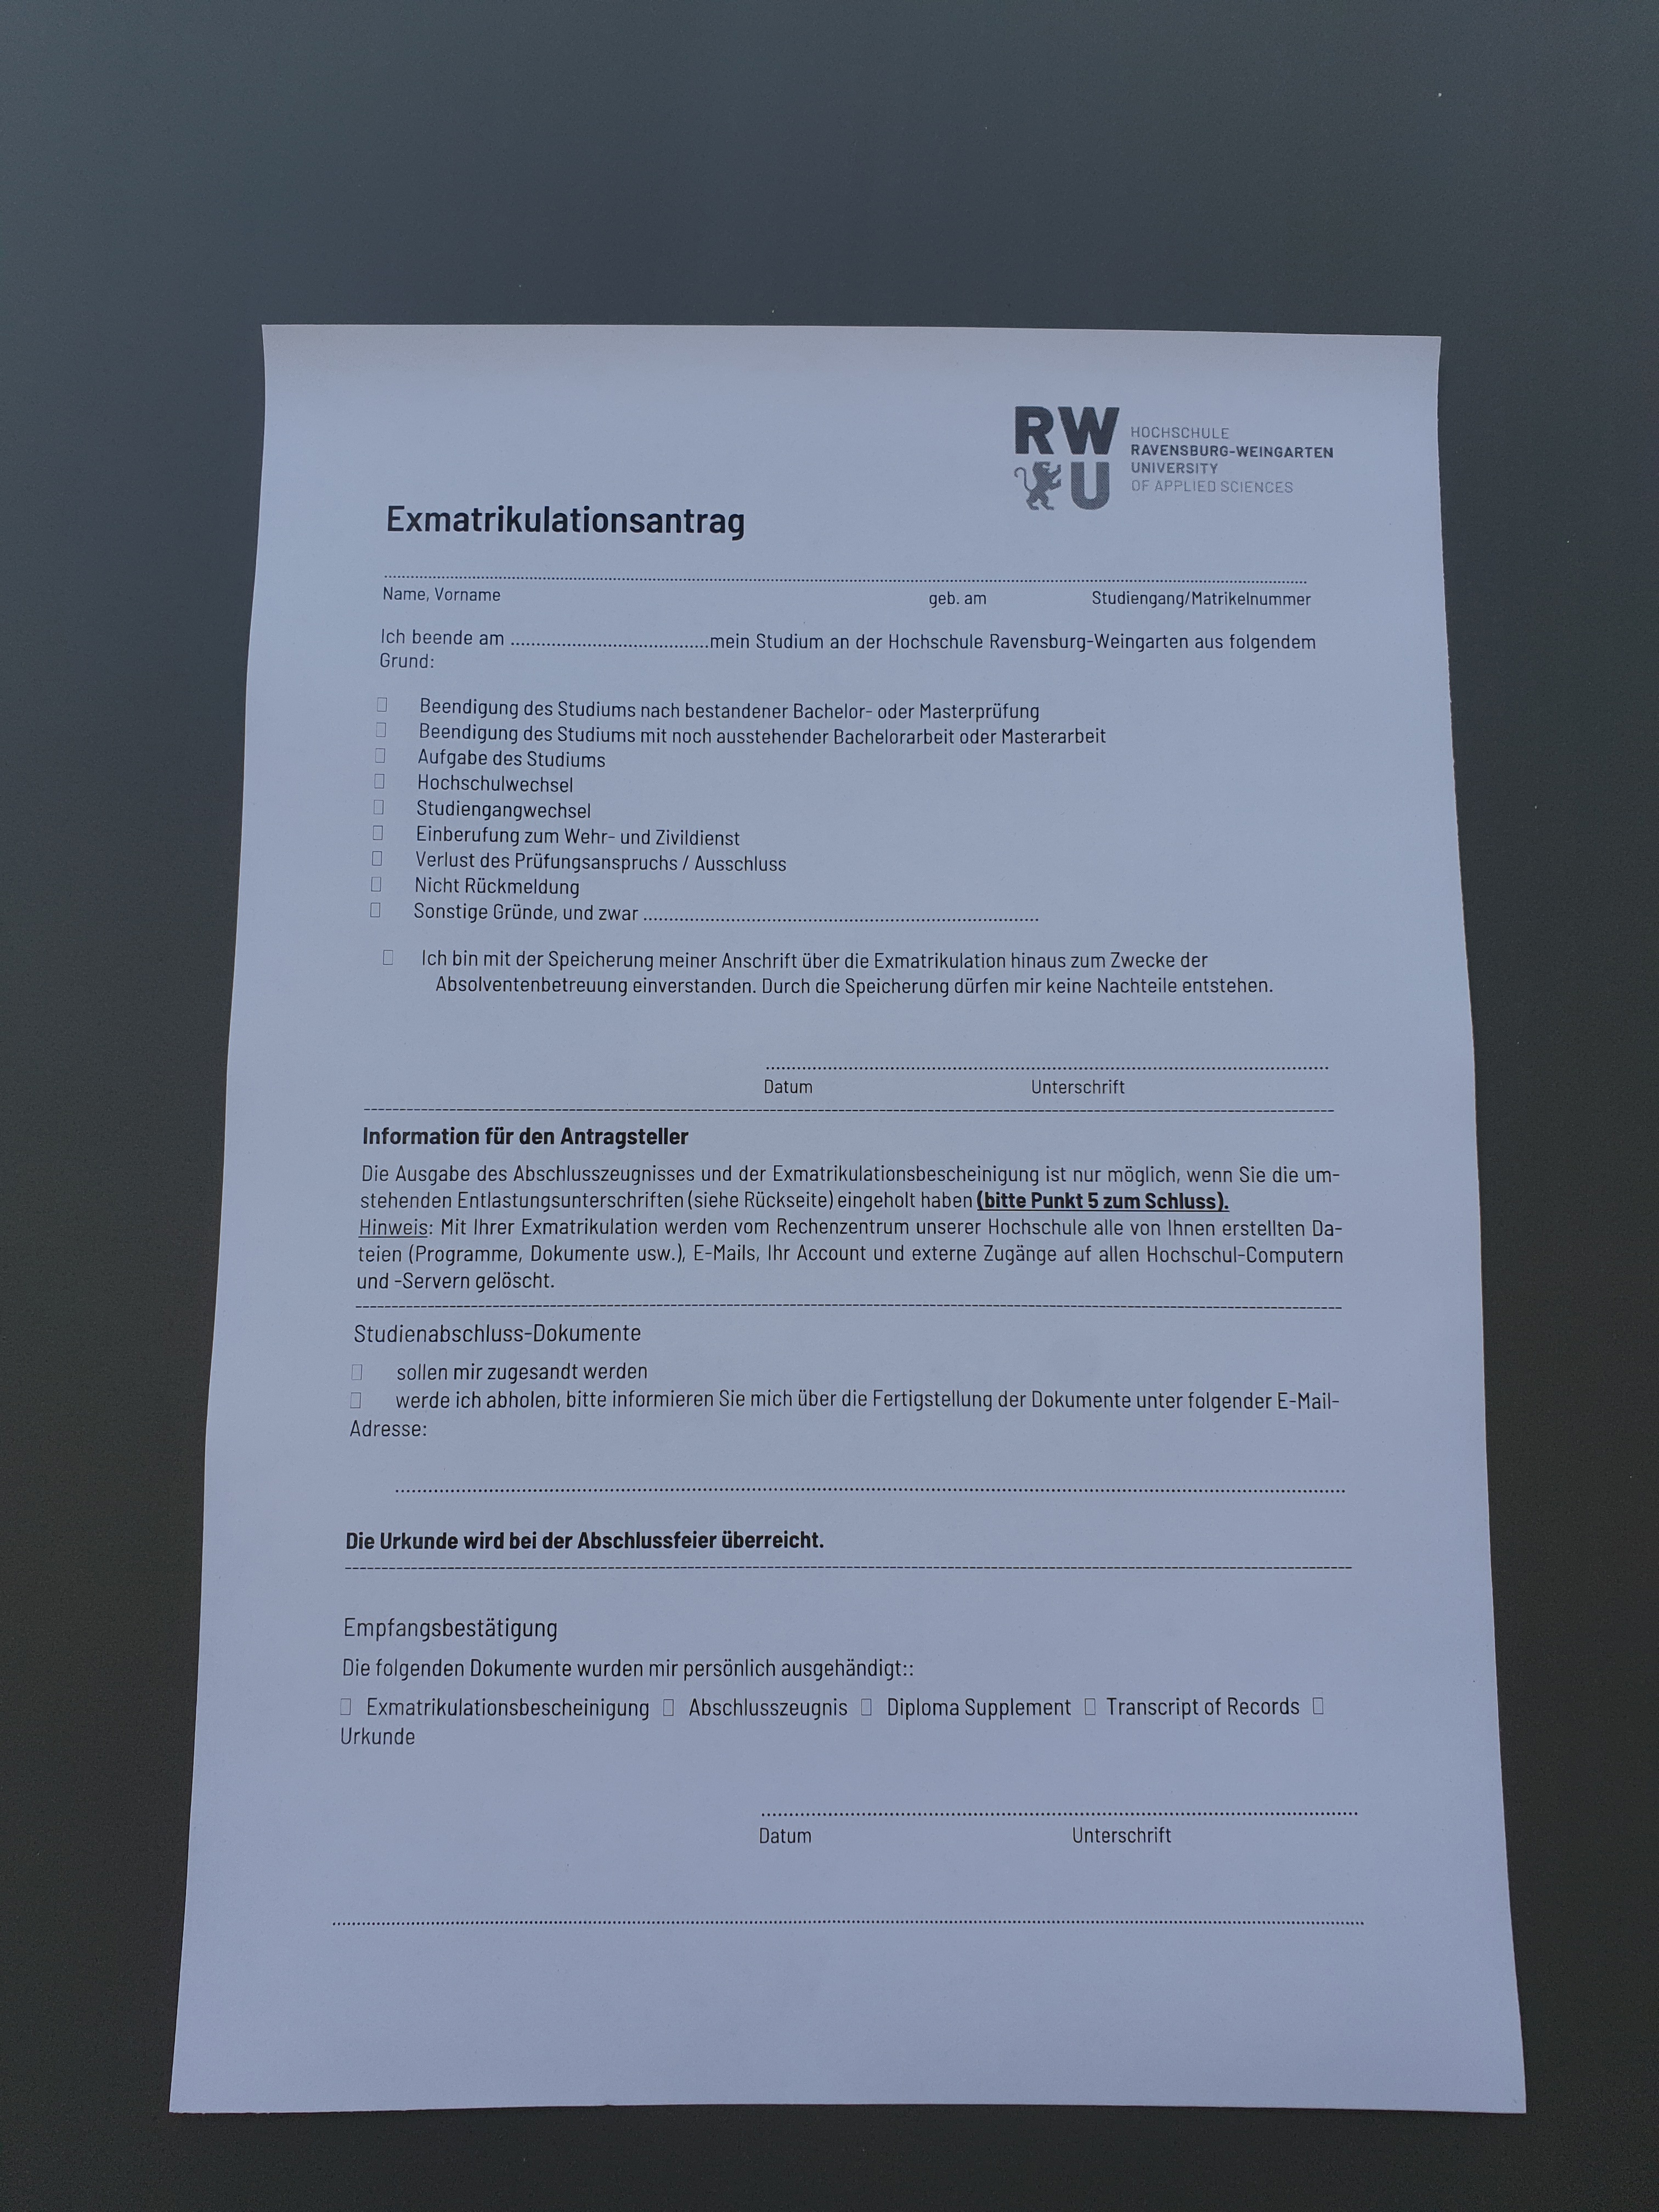
\includegraphics[width=2.5in]{output/hoch_3_1_original.jpg}}
    \caption{Original image.}
    \label{fig:orginial}
\end{figure}
\noindent
For further steps the photo is needed in a grayscale format (Figure \ref{fig:grayscale}).
This convertion is made with the cvtColor\cite{opencv_cvtColor} function of OpenCV. The convertion of colorspace is made with the following
formula\cite{opencv_rgb2gray}:
\begin{center}
    $Y = B * 0.114 + G * 0.587 + R * 0.299$
    \label{eq_rgb2gray}
\end{center}
\begin{center}
    \noindent
    $cvtColor(image,COLOR_BGR2GRAY)$
\end{center}
\noindent
\begin{figure}[H]
    \centerline{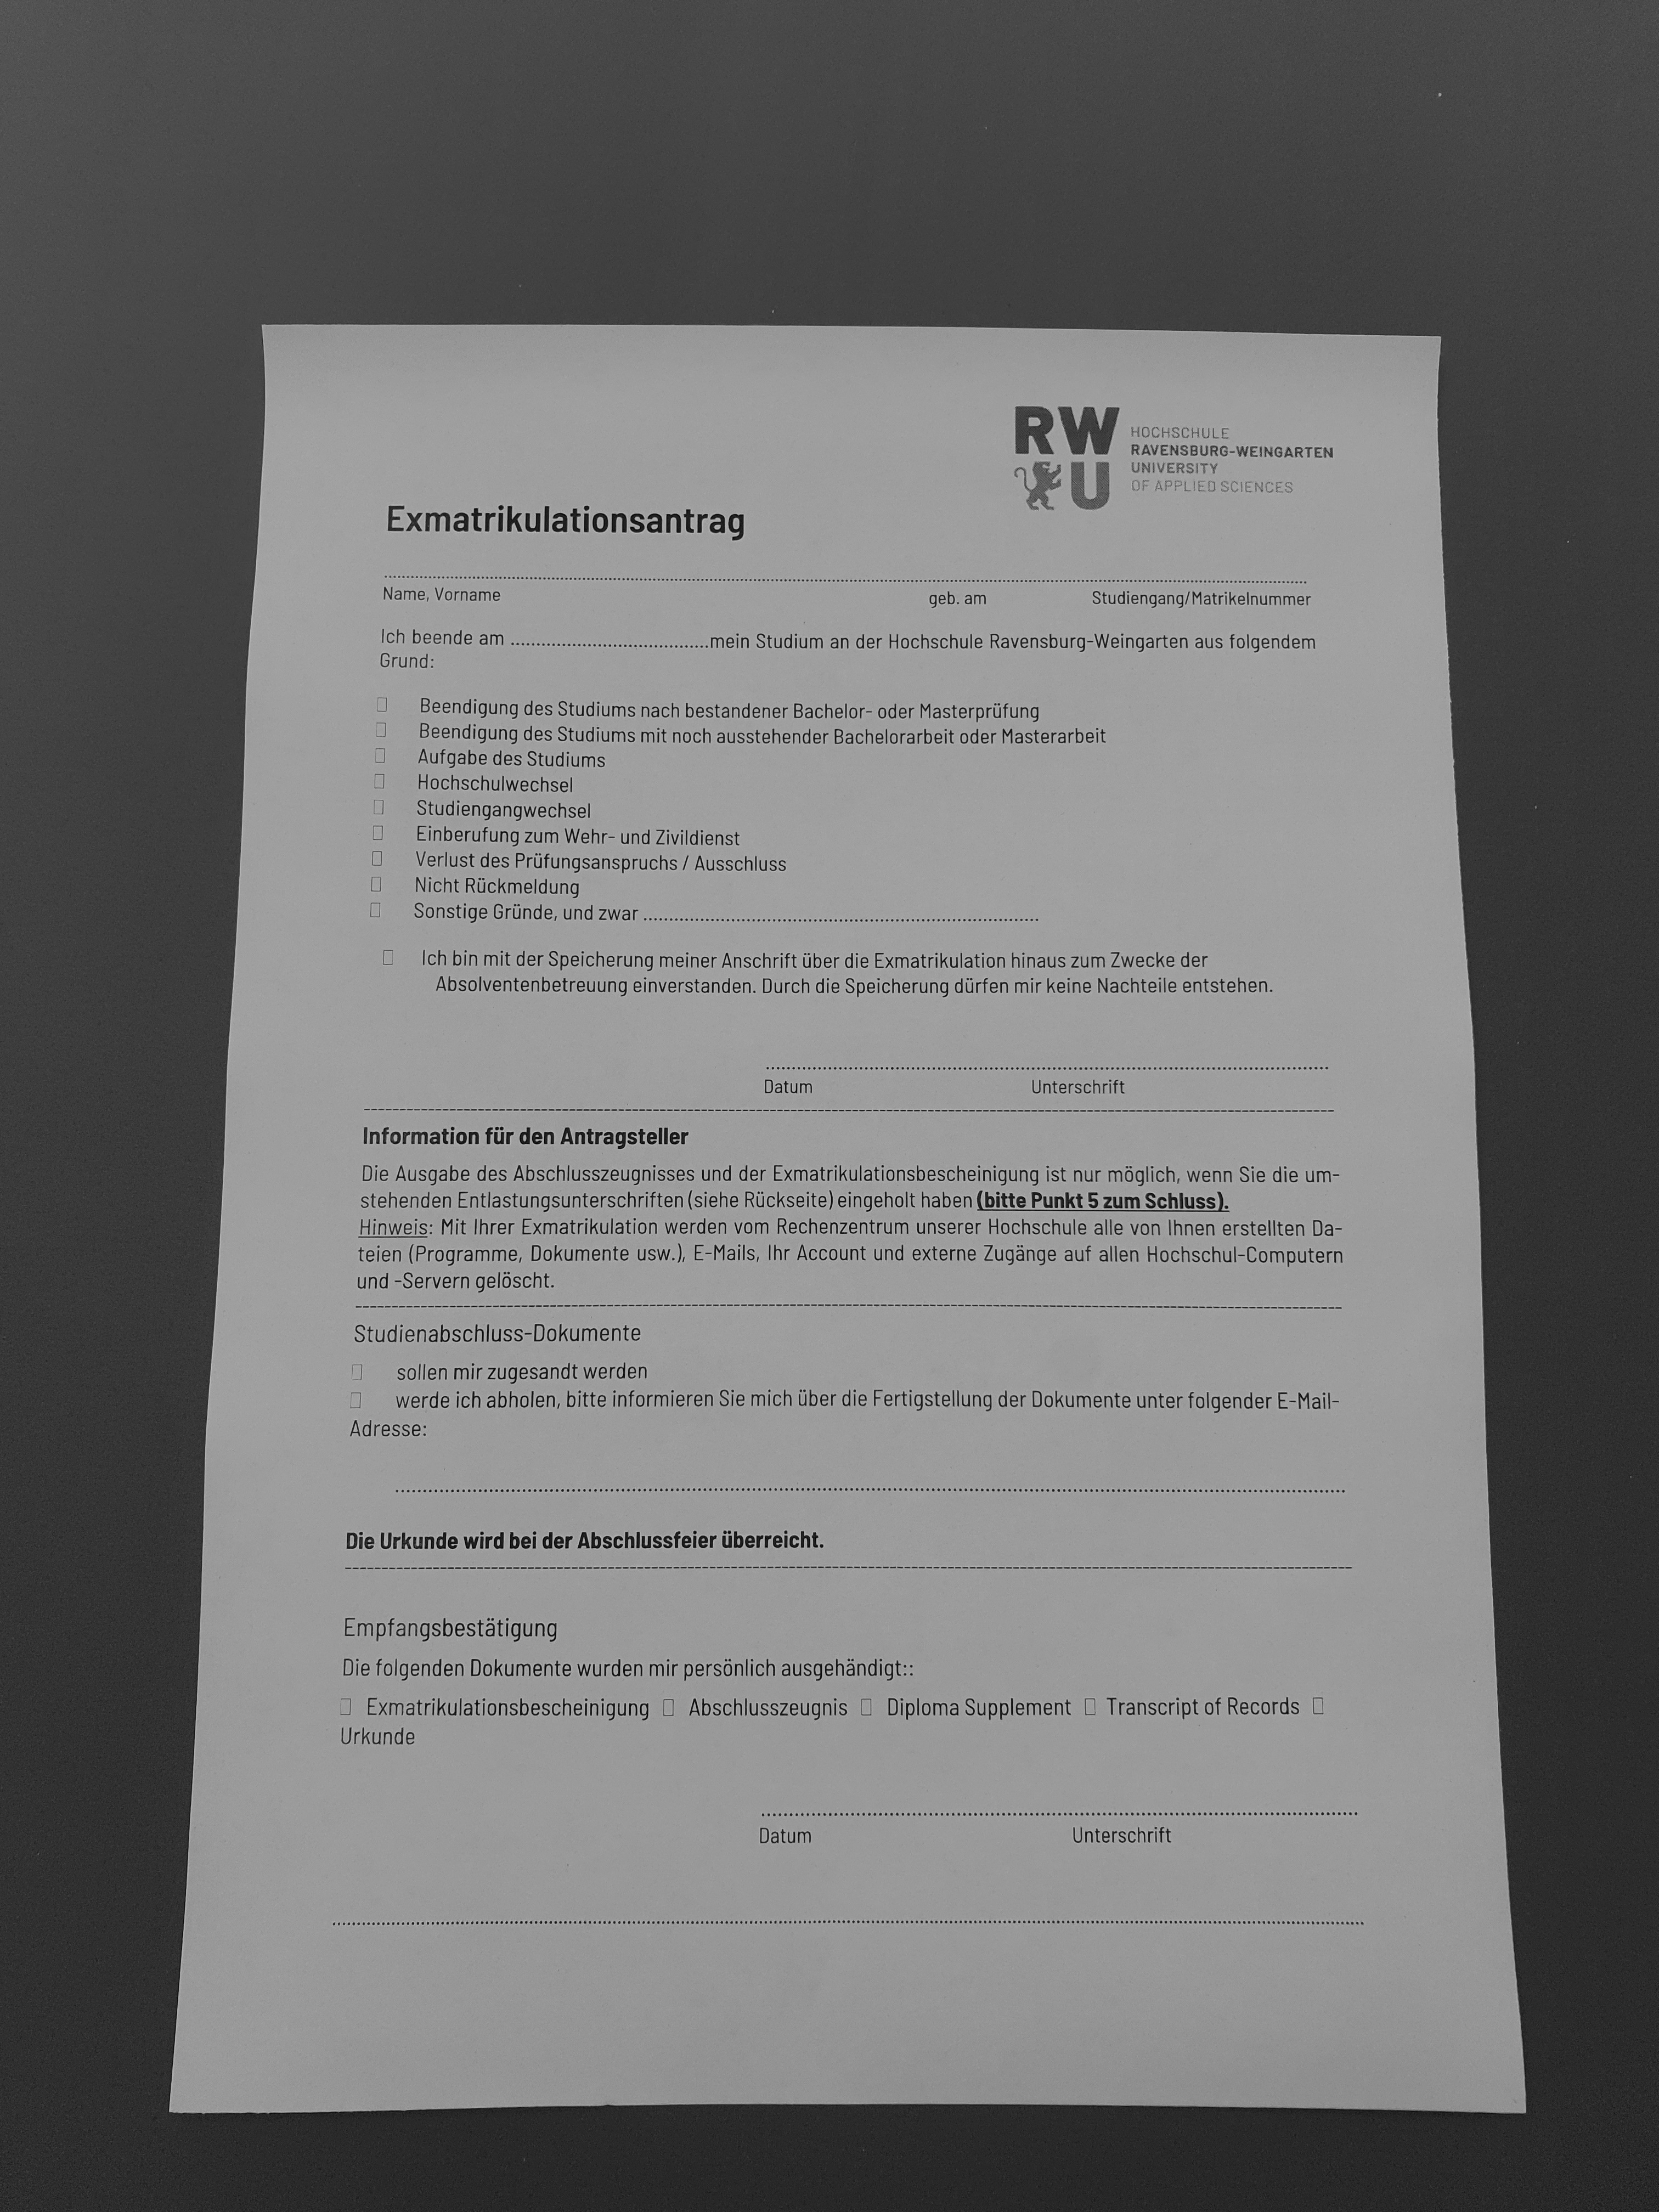
\includegraphics[width=2.5in]{output/hoch_3_2_grayscaleimg.jpg}}
    \caption{Grayscale image.}
    \label{fig:grayscale}
\end{figure}
The next preprocessing step includes the blurring of the grayscale image.
This is done to remove noise from the image\cite{opencv_smoothingimages}. In this case
the Gaussian Blurring\cite{opencv_gaussianblur} is used. There the image is convolved with the Gaussian Kernel.
As size of the kernel the size (5,5) is used.
Because a document could be landscape or portrait format, 
it makes sense to use same values in x and y direction in the kernel size, as well as for the parameters
sigmaX and sigmaY.
The optimum values of these parameters were determined from the results of several scans of sample documents.
The parameters sigmaX and sigmaY are used to calculate the gaussian filter coefficients. In the function call
sigmaX and sigmaY are set to zero, which means the Gaussian Kernel computes these variables from the given
ksize\cite{opencv_getgaussiankernel}.
\begin{center}
    $\sigma = 0.3 * (0.5 * (ksize - 1 ) - 1) + 0.8$
    \label{eq_sigma}
\end{center}
The gaussian filter coefficients are computated with the following formula\cite{opencv_getgaussiankernel}:
\begin{center}
    $G_i = \alpha * e^{- \frac{(i - \frac{(ksize - 1)}{2})^2}{2*\sigma^2 } }$
    \label{eq_sigma}
\end{center}
\begin{center}
    \noindent
    $GaussianBlur(grayscale_image, ksize=(5,5),sigmaX=0,sigmaY=0)$
\end{center}
\noindent
\begin{figure}[H]
    \centerline{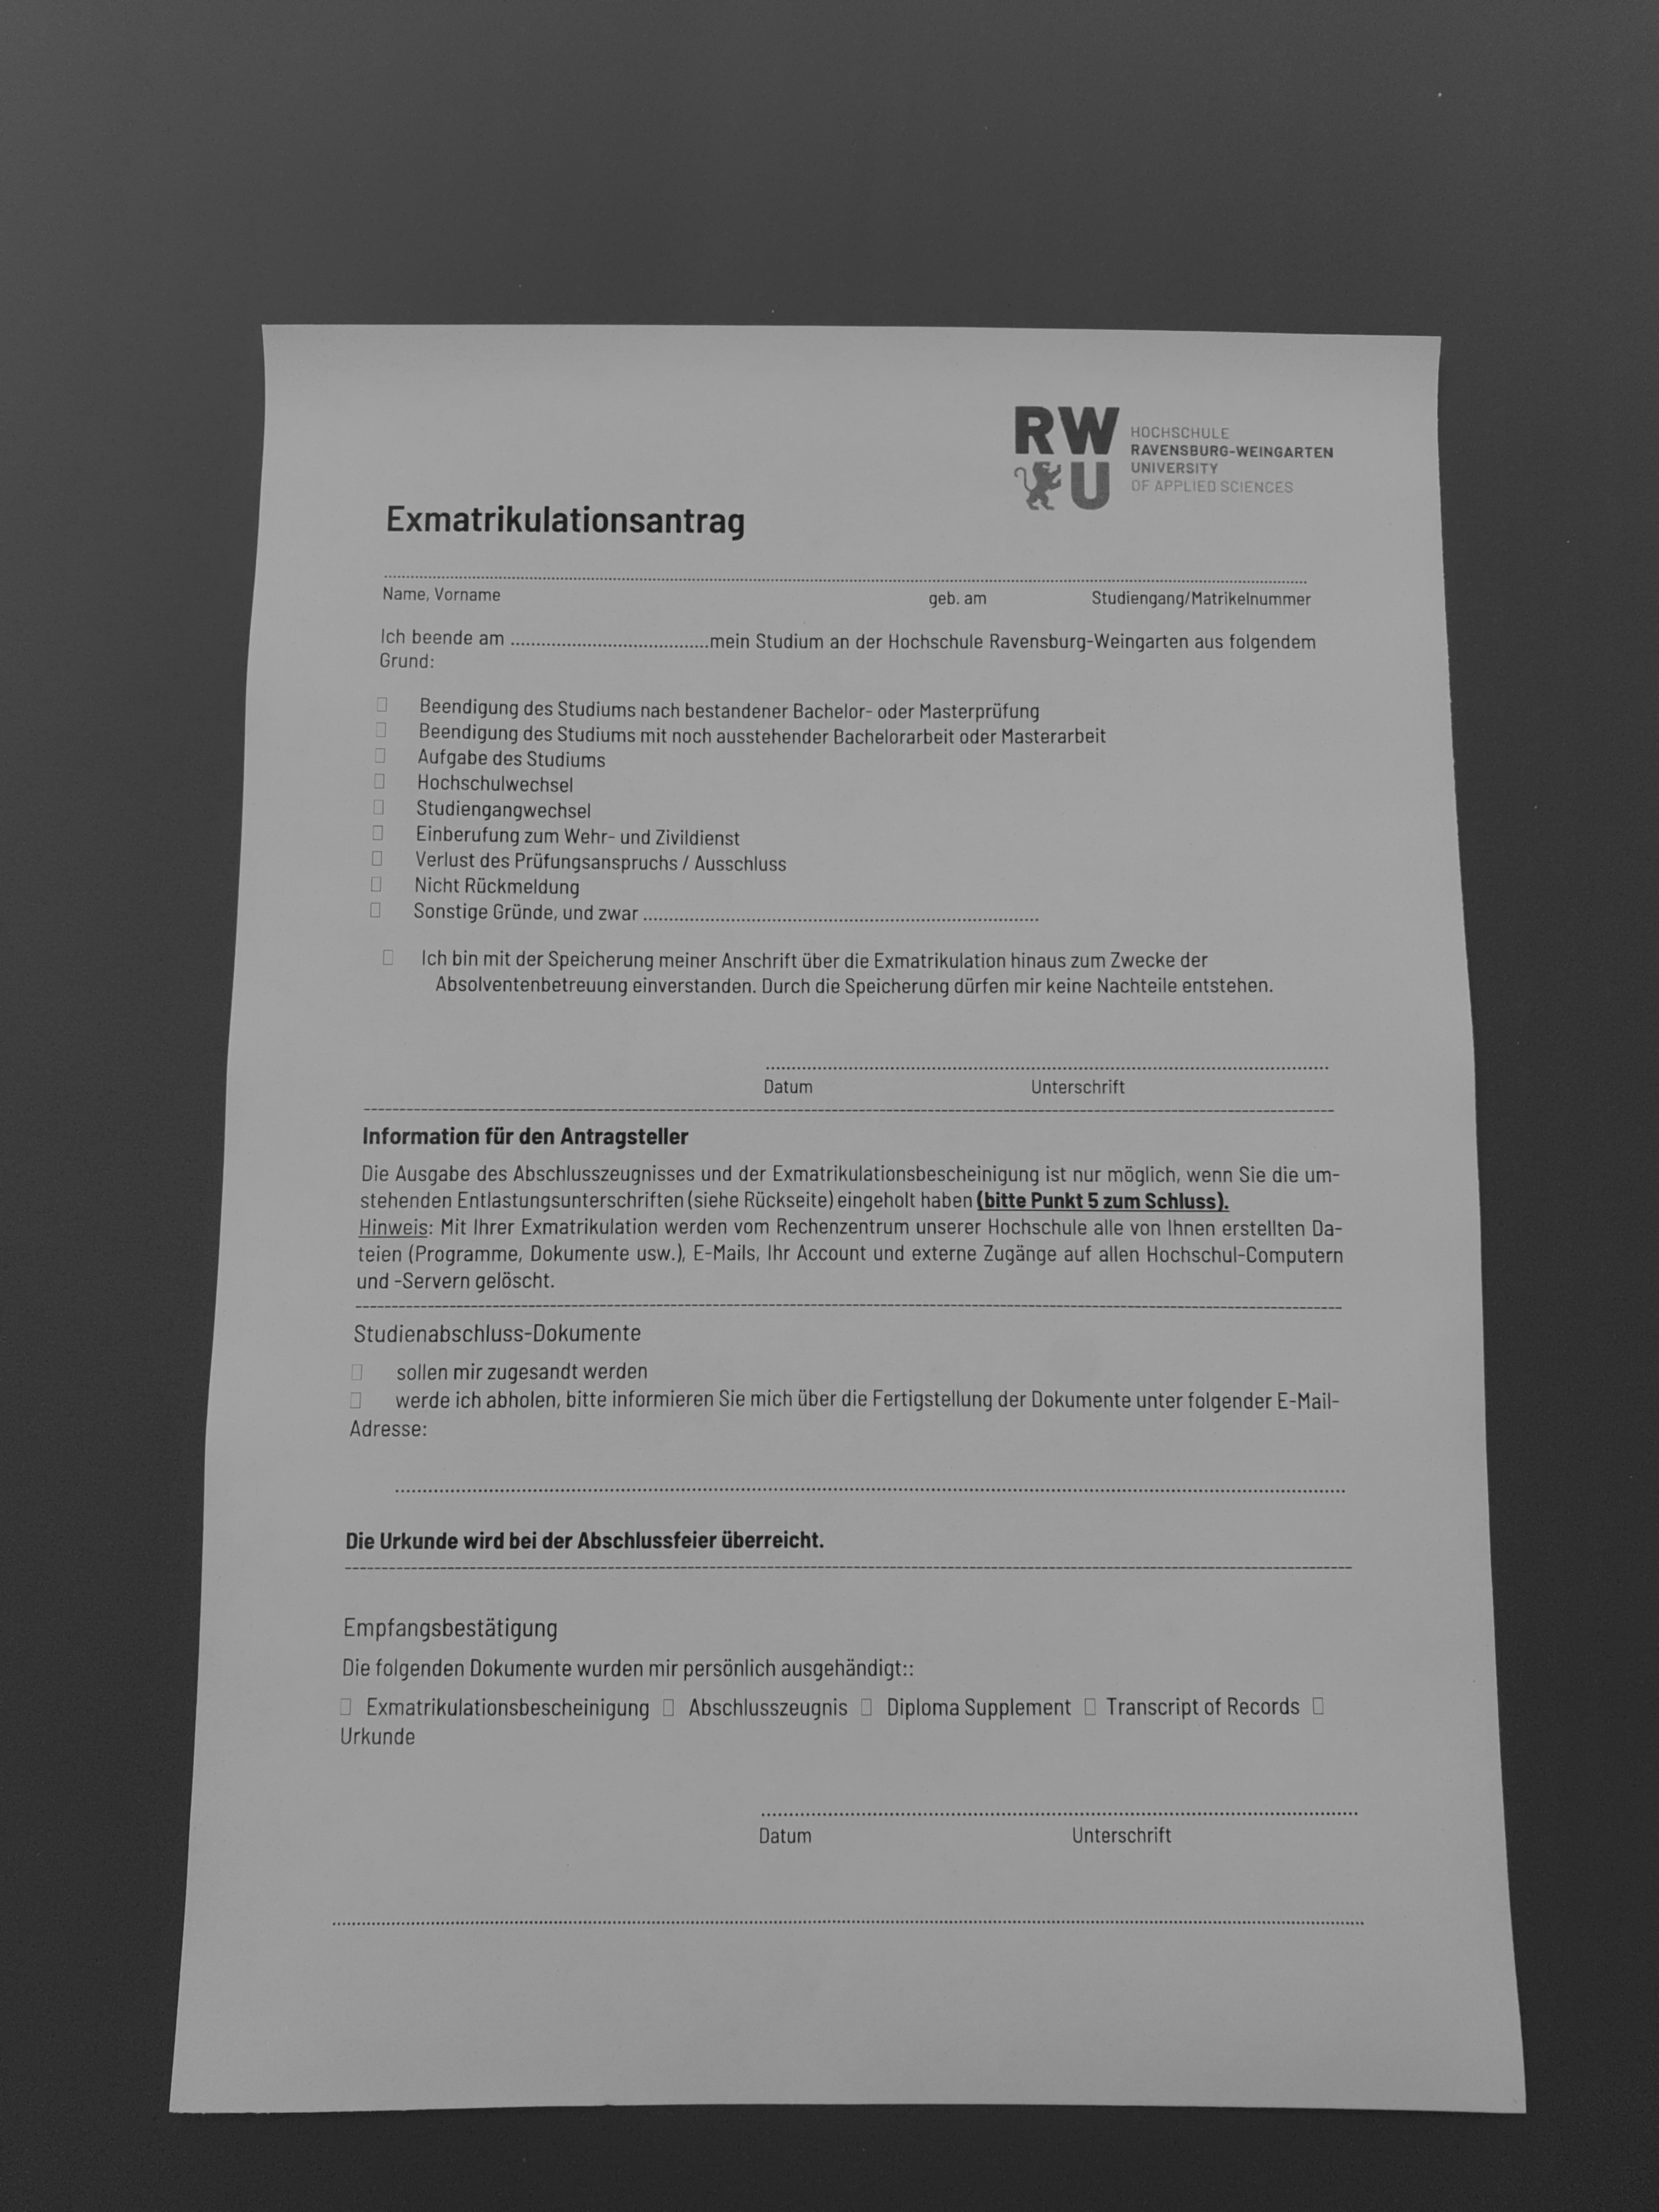
\includegraphics[width=2.5in]{output/hoch_3_3_gaussianblur.jpg}}
    \caption{Grayscale image with Gaussian Blur.}
    \label{fig:grayscale}
\end{figure}
% The heading is boldface with upper and lower case letters. 
% If the heading should run into more than one line, the run-over is not left-flushed.

%%%%%%%%%%%%%%%%%%%%%%%%%%%%%%%%%%%%%%%%%%%%%%%%%%%%%%%%%%%%%%%%%%%%%%
\section{Edge Detection}
\label{section:edgedetection}
% edges = Canny(blurred_image,75,180, L2gradient=True)
\noindent
After preprocessing steps are taken and a suitable noise reduction algorithm was chosen, the edge detection can be started.
For edge detection the Canny edge\cite{canny_paper} detector is used, which is a multi-staged algorithm:
\begin{enumerate}
    \item Noise reduction.
    \item Calculating the intensity gradient of the image.
    \item Non-maximum supression.
    \item Hysteresis thresholding.
\end{enumerate}
The noise reduction step was already described in the \nameref{section:preprocessing} section of this paper.
\\\\
The intensity gradient of the image is calculated using the \textbf{Sobel Filter}:
\begin{equation}
    S(I(x,y)) :=\sqrt{(S_x*I(x,y))^2 + S_y(*I(x,y))^2}
\end{equation}
Generally we can define the gradient of the Image I as:
\begin{equation}
    G(I(x,y)) := \sqrt[]{I_x^2 +I_y^2}
\end{equation}
\noindent
In addition to the gradient we calculate the the orientation given by:
\begin{equation}
    \phi(x,y) = arctan(\frac{g_y}{g_x})
\end{equation}

\noindent
After getting the gradient magnitude and orientation of each pixel, the edges have
to be reduced to a thickness of one pixel which will be realized with \textbf{non-maximum supression.}
\\
Lastly it is decided whether a pixel will be mapped to 1 or 0 with application of \textbf{hysteresis.}\\\\
\noindent
To implement this method in the document scanner, the function
which implements the full Canny edge detector\cite{opencv_canny} can be called:
\begin{center}
    \noindent
    $Canny(blurred\_image,75, 180,$\\
    $L2gradient = True, apertureSize = 3)$
\end{center}
\noindent
The functions input is the noise reduced image described in \nameref{section:preprocessing}.
For Hysteresis Threshold 75 for the lower-bound and 180 for the upper bound are chosen.
In several trials this settings could sufficiently provide the overall best results 
when setting the aperture size to 3.
Instead of the predefined L1-Norm \cite{l1_norm}, the more precise L2-Norm\cite{l2_norm} is used.
\\\\
The Canny edge detection filter returns an binary output image with edges
being set to 1 and other points being set to 0.
\\\\
This can be seen in Figure \ref{fig:canny}

\begin{figure}[H]
\centerline{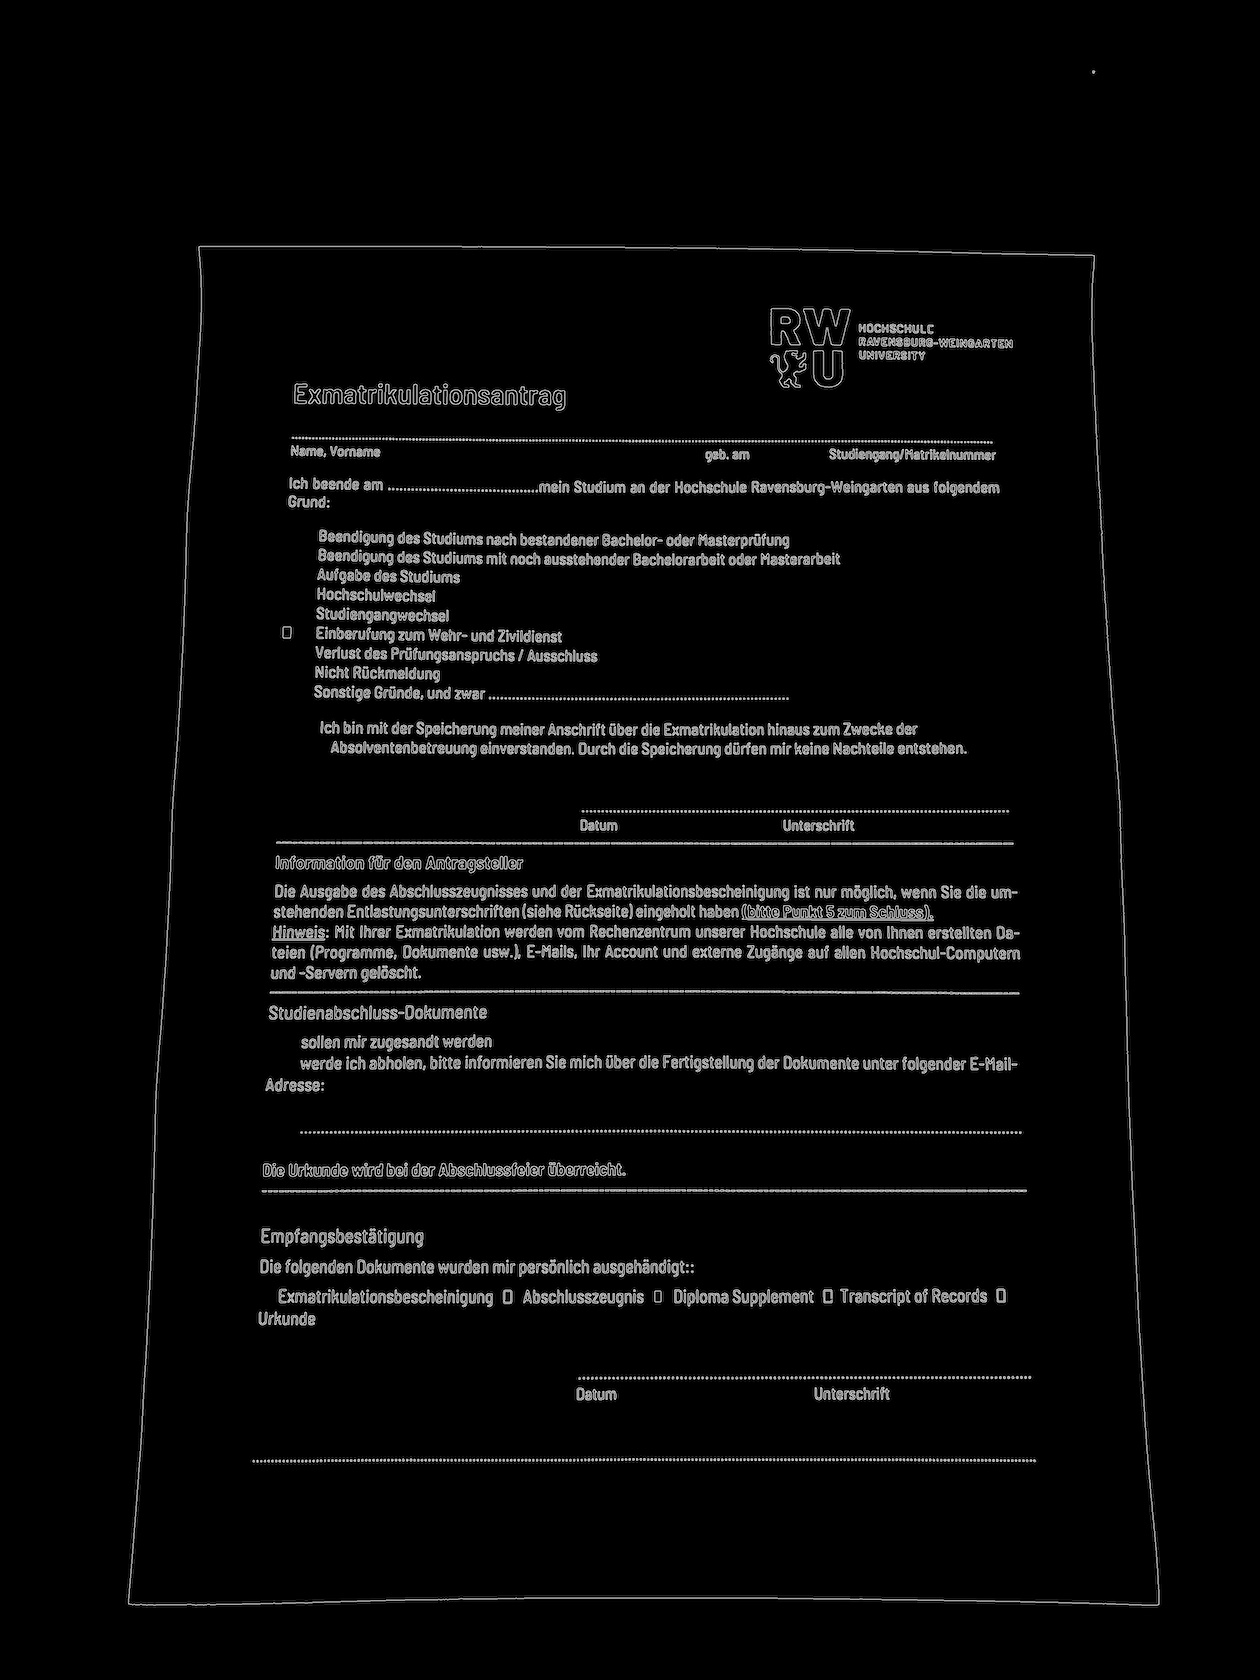
\includegraphics[width=2.5in]{output/hoch_3_4_canny.jpg}}
\caption{The output image of the Canny edge detection.}
\label{fig:canny}
\end{figure}

%%%%%%%%%%%%%%%%%%%%%%%%%%%%%%%%%%%%%%%%%%%%%%%%%%%%%%%%%%%%%%%%%%%%%%
\section{Corner Detection}
\noindent
To find the corner of the document the previously generated edges 
in \nameref{section:edgedetection} have to be evaluated.
For this purpose, contours are formed which are represented by a curve that connects all 
continuous points with each other\cite{SUZUKI198532}.\\\\
\noindent
The OpenCV function\cite{opencv_findcontours} is used as follows:
\begin{center}
    \noindent
    $findContours(edges,$\\
    $RETR\_LIST, CHAIN\_APPROX\_SIMPLE)$
\end{center}
\noindent
Where the input are the previously generated edges, the retrieval 
mode\cite{opencv_retrievalmode} which is 
set to retrieve the contours without establishing any hierarchical relationships 
and the contour approximation mode\cite{opencv_approxmode} which is set to ouput only their endopints.
(E.g: A rectengular contour is defined by the four corner points)
This can be seen in Figure \ref{fig:contours}\\\\
\noindent
The assumption is made that the document is the largest polygon in the image.
The contours are hierarchically sorted according to their area, with the largest polygon with four vertices being selected.

\begin{figure}[H]
\centerline{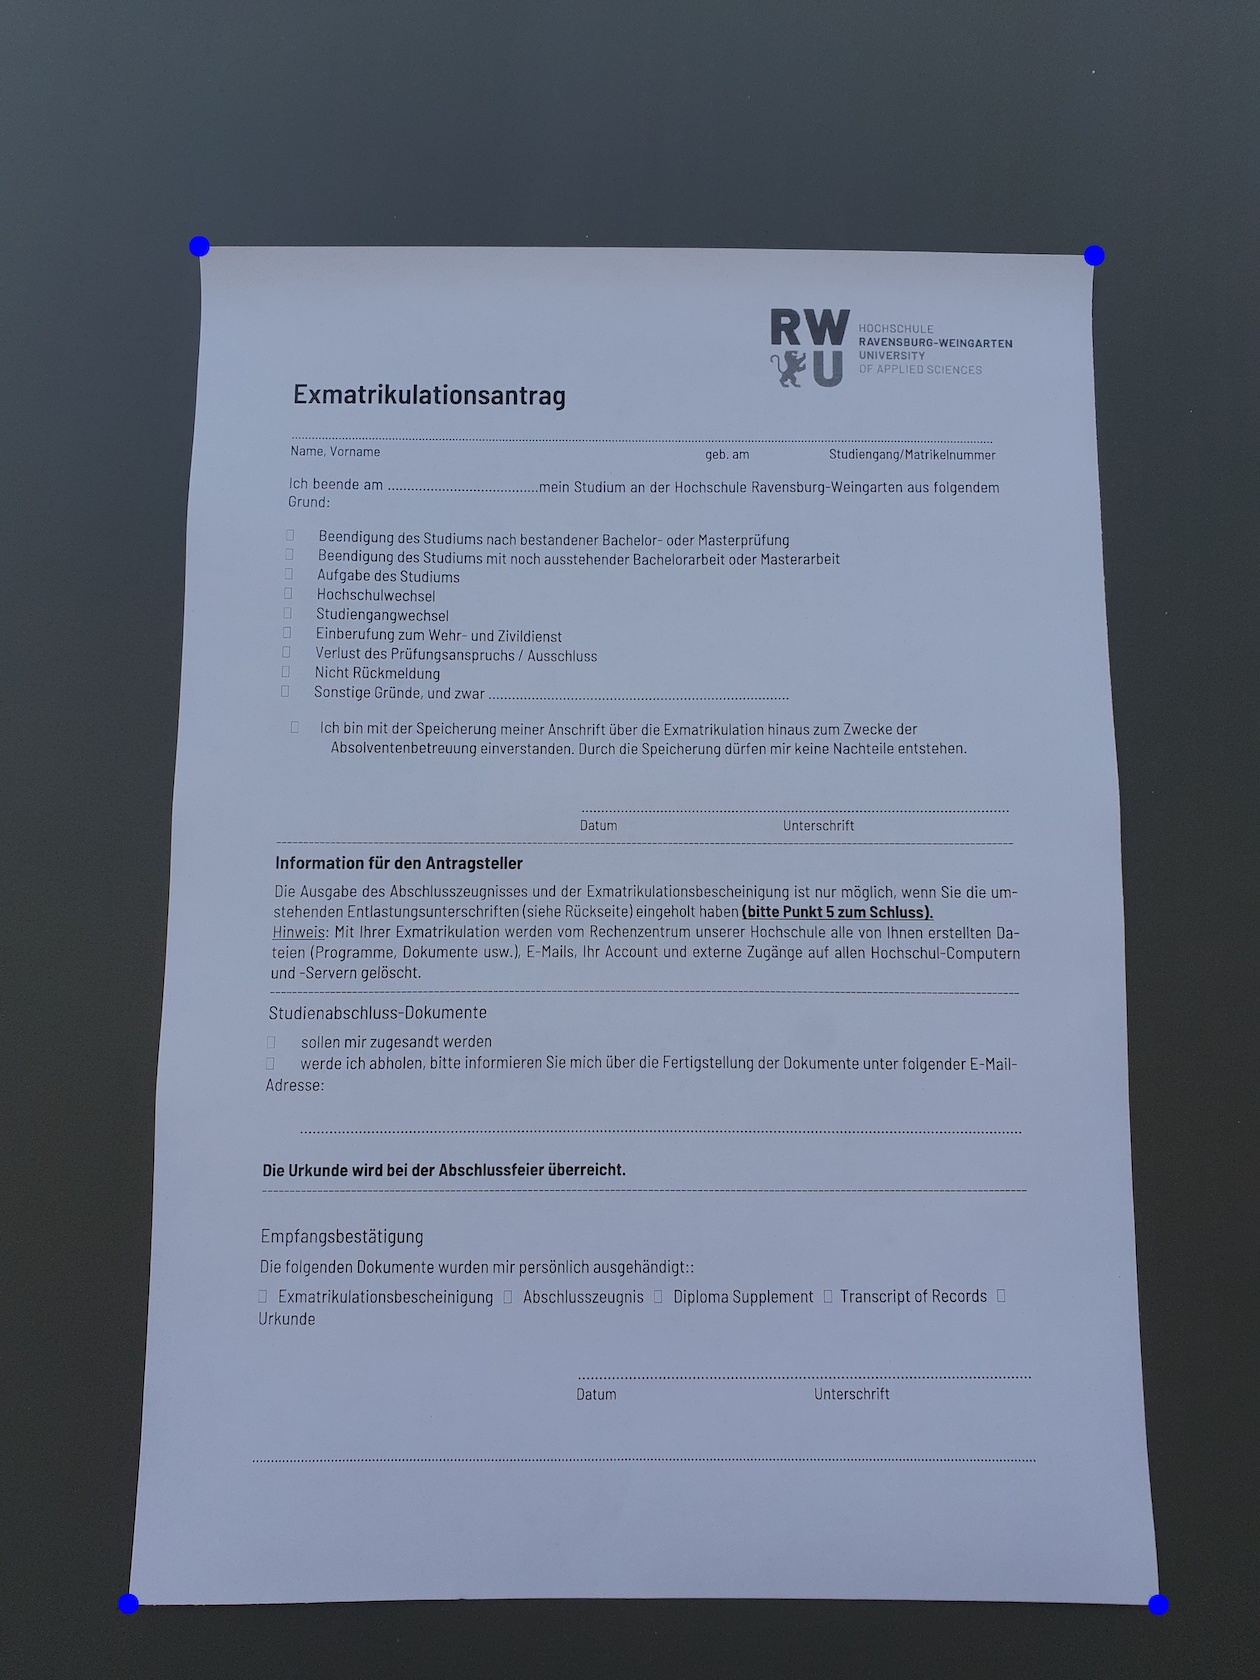
\includegraphics[width=2.5in]{output/hoch_3_5_contouredimage.jpg}}
\caption{The corners of the document.}
\label{fig:contours}
\end{figure}

% Appox Poly
\cite{doi:10.3138/FM57-6770-U75U-7727}
\cite{RAMER1972244}


% findContours
% Paper:
% https://reader.elsevier.com/reader/sd/pii/0734189X85900167?token=11C96FBB310332A0D41181ED5B29CA355D79630C93940FA6DCEABD7D12A580B1F46464823FDA2CB7D695CA063C30B005&originRegion=eu-west-1&originCreation=20220509094855
% contours = sorted(contours, key=contourArea, reverse=True)
%epsilon = 0.1*arcLength(contour,True)
%approx = approxPolyDP(contour,epsilon,True)


\section{Transformation}
\label{section:transformation}
\noindent
% def order_points(pts):    
%     print(pts)
%     a = np.sum(np.square(pts[0,0]-pts[1,0]))
%     b = np.sum(np.square(pts[0,0]-pts[3,0]))

%     if a > b:
%         rect = pts.copy()
%         rect[0] = pts[0]
%         rect[1] = pts[3]
%         rect[2] = pts[2]
%         rect[3] = pts[1]
%         return rect
%     else:
%         rect = pts.copy()
%         rect[0] = pts[1]
%         rect[1] = pts[0]
%         rect[2] = pts[3]
%         rect[3] = pts[2]
%         return rect

% h = 3000
%     w = int(np.floor(h*(1/np.sqrt(2))))
%     dst_pts = np.array([[0, 0],   [w-1, 0],  [w-1, h-1], [0, h-1]], dtype=np.float32)
%     src_pts = np.array(order_points(doc_cnts), dtype=np.float32).reshape(4,2)
%     M = cv2.getPerspectiveTransform(src_pts, dst_pts)
% transformation = cv2.warpPerspective(grayscale_image, M, (w, h))

Before the transformation can be performed the orientation of the document in the image must be found out.
Without knowing the content of the document, it is not possible to know the real orientation. Therefore a few assumptions are made:
\begin{itemize}
    \item[1.] All provided documents are in ISO 216 format
    \item[2.] All provided documents are portrait format
    \item[3.] All provided documents are only rotated 90 degrees right or left, otherwise the document is scanned upside down.
\end{itemize}
These assumptions define the output of the scanner: A document in portrait format.
The first task is to find out if the document is landscape or portrait in the image.
Four examples of how the document could have been recorded can be seen in Figure \ref{fig:fourcorners}.
What is known from the list of the given four corners from the previous section is that the first element \bluecircled{-} is the most upper point in the image. 
Next, the distance of this point must be calculated with the second and fourth elements \redcircled{-} in the list and these two distances compared. For this purpose, the Euclidean distance calculation is used. If the distance to the second element is higher than to the fourth element, the document is recorded portrait. Otherwise it was recorded landscape. 
Relative to the previous result, the list of found points must be put into this form:
\begin{center}
    \noindent
    $[\textrm{upper\_left}, \textrm{upper\_right}, \textrm{lower\_right}, \textrm{lower\_left}]$
\end{center}
This is used to calculate the perspective transformation from the given points to the destination points with the getPerspectiveTransform\cite{opencv_getPerspectiveTransform} function from OpenCV. 
The target points are the set points of the document in ISO 216 format.
\begin{center}
    \noindent
    $[[0,0], [\textrm{width},0], [\textrm{width},\textrm{height}], [0,\textrm{height}]]$\\
    $\textrm{height}=3000$\\
    $\textrm{width}=\frac{\textrm{height}}{\sqrt[2]{2}}$
\end{center}
\begin{figure}[H]
    \centerline{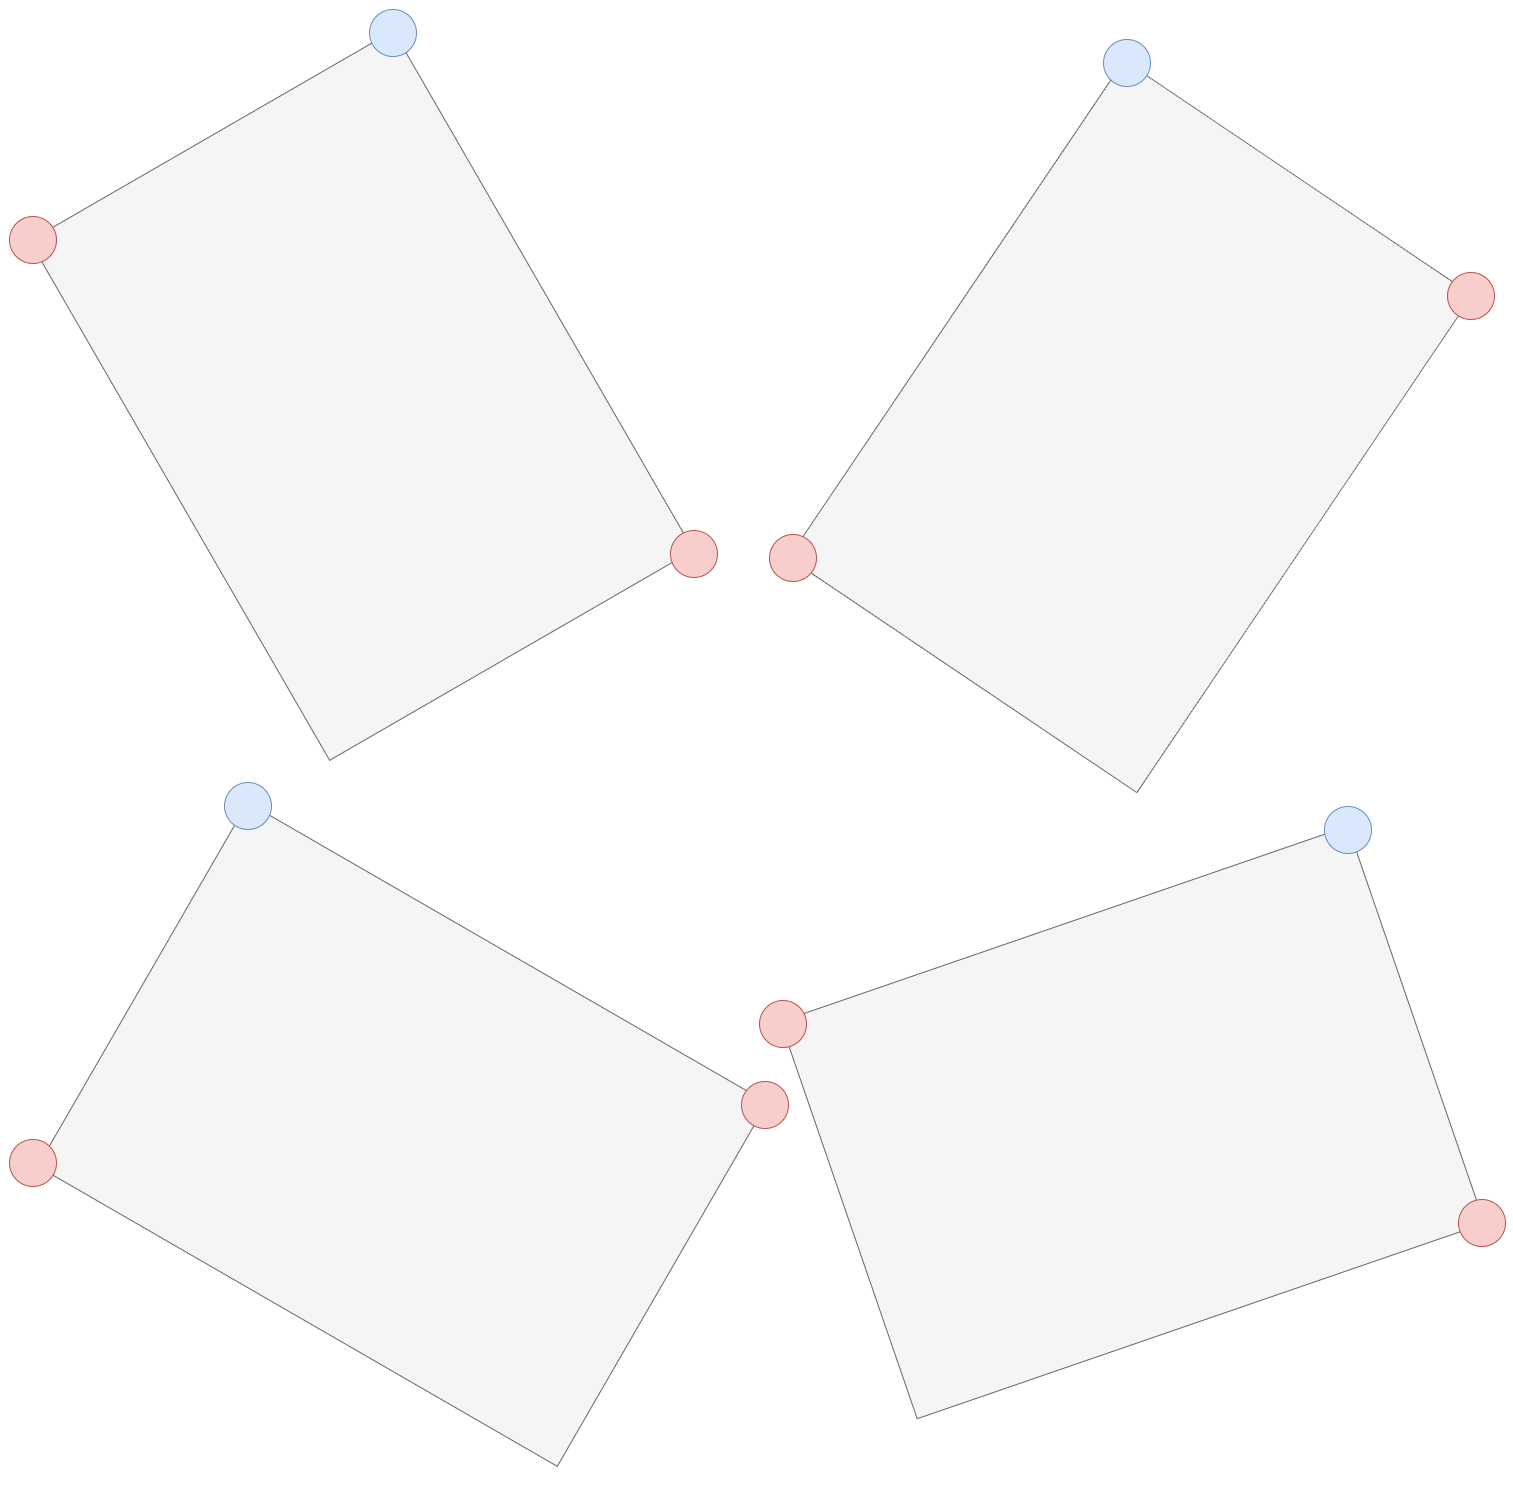
\includegraphics[width=2.5in]{output/a.png}}
    \caption{Four examples of the orientation of a scanned document}
    \label{fig:fourcorners}
\end{figure}
\begin{center}
    \noindent
    $getPerspectiveTransform(src_pts, dst_pts)$
\end{center}
The last step of this section is to apply the perspective transformation to the grayscale image. 
For this purpose the warpPerspective function\cite{opencv_warpPerspective} from OpenCV is used:
\begin{center}
    \noindent
    $warpPerspective(grayscale\_image, M, (width, height))$
\end{center}
The function uses the grayscale image, the calculated perspective Transformation(M), and the size of the 
output image to perform the transformation. The optional parameters are set to default.
The output of the transformation can be seen in Figure \ref{fig:transformation}.

\begin{figure}[H]
    \centerline{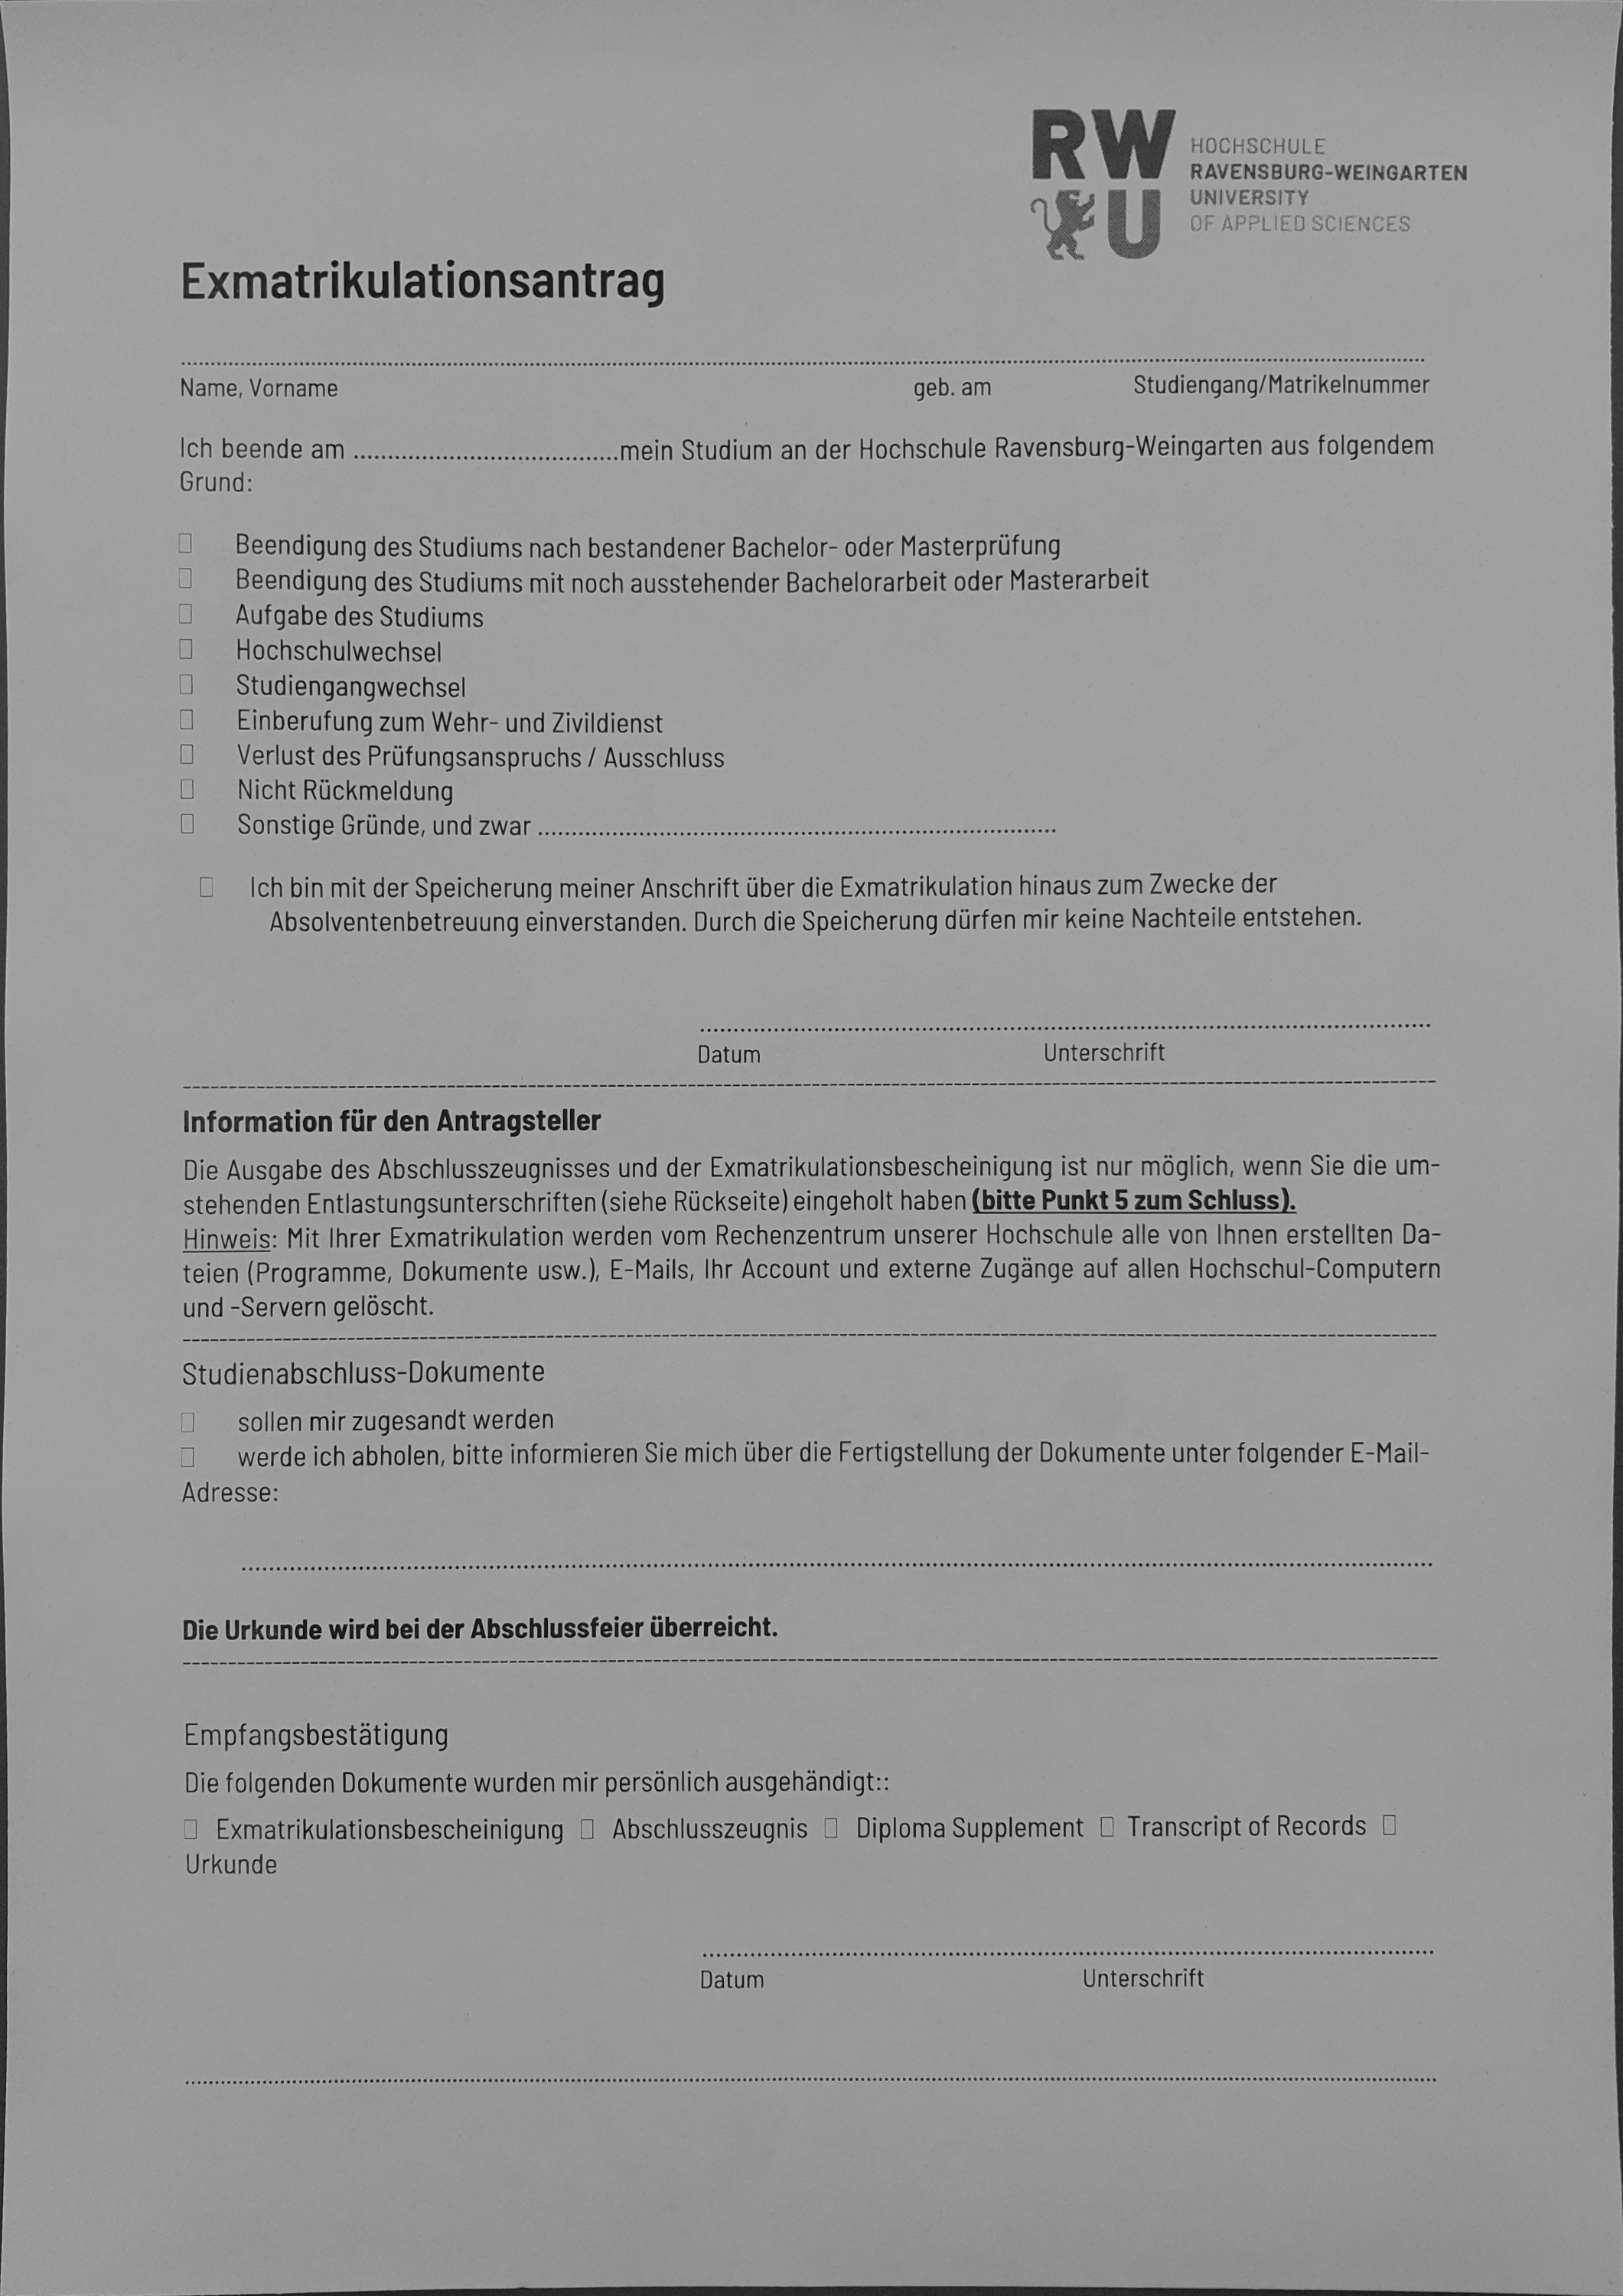
\includegraphics[width=2.5in]{output/hoch_3_6_transformation.jpg}}
    \caption{Document after the transformation.}
    \label{fig:transformation}
\end{figure}




\section{Binary Image}
% adaptive_binary_image = adaptiveThreshold(transformation,255,ADAPTIVE_THRESH_GAUSSIAN_C, THRESH_BINARY,11,6)
%tresh, binary_image = threshold(transformation, 100,255,THRESH_BINARY)
\noindent
In the last step of the process, the transformed image is converted into a binary image.
In various tests, it has been found that an adaptive threshold\cite{opencv_adaptivethreshold} is best suited.
Both an adaptive gaussian threshold\cite{pencv_adaptivetypes} and an adaptive mean threshold show great performance, 
though an adaptive mean threshold tends to generate less noise in the outputs.

\begin{center}
    \noindent
    $adaptive\_binary\_image\_mean = $\\
    $adaptiveThreshold(transformation,255,$\\
    $ADAPTIVE\_THRESH\_MEAN\_C, $\\
    $THRESH\_BINARY,7,6)$
\end{center}
\noindent

The chosen adaptive mean threshold value is a mean of the blocksize $7*7$ minus the constant $c=6$.
The image generated after this process can be seen in figure \ref{fig:binary}

\begin{figure}[H]
    \centerline{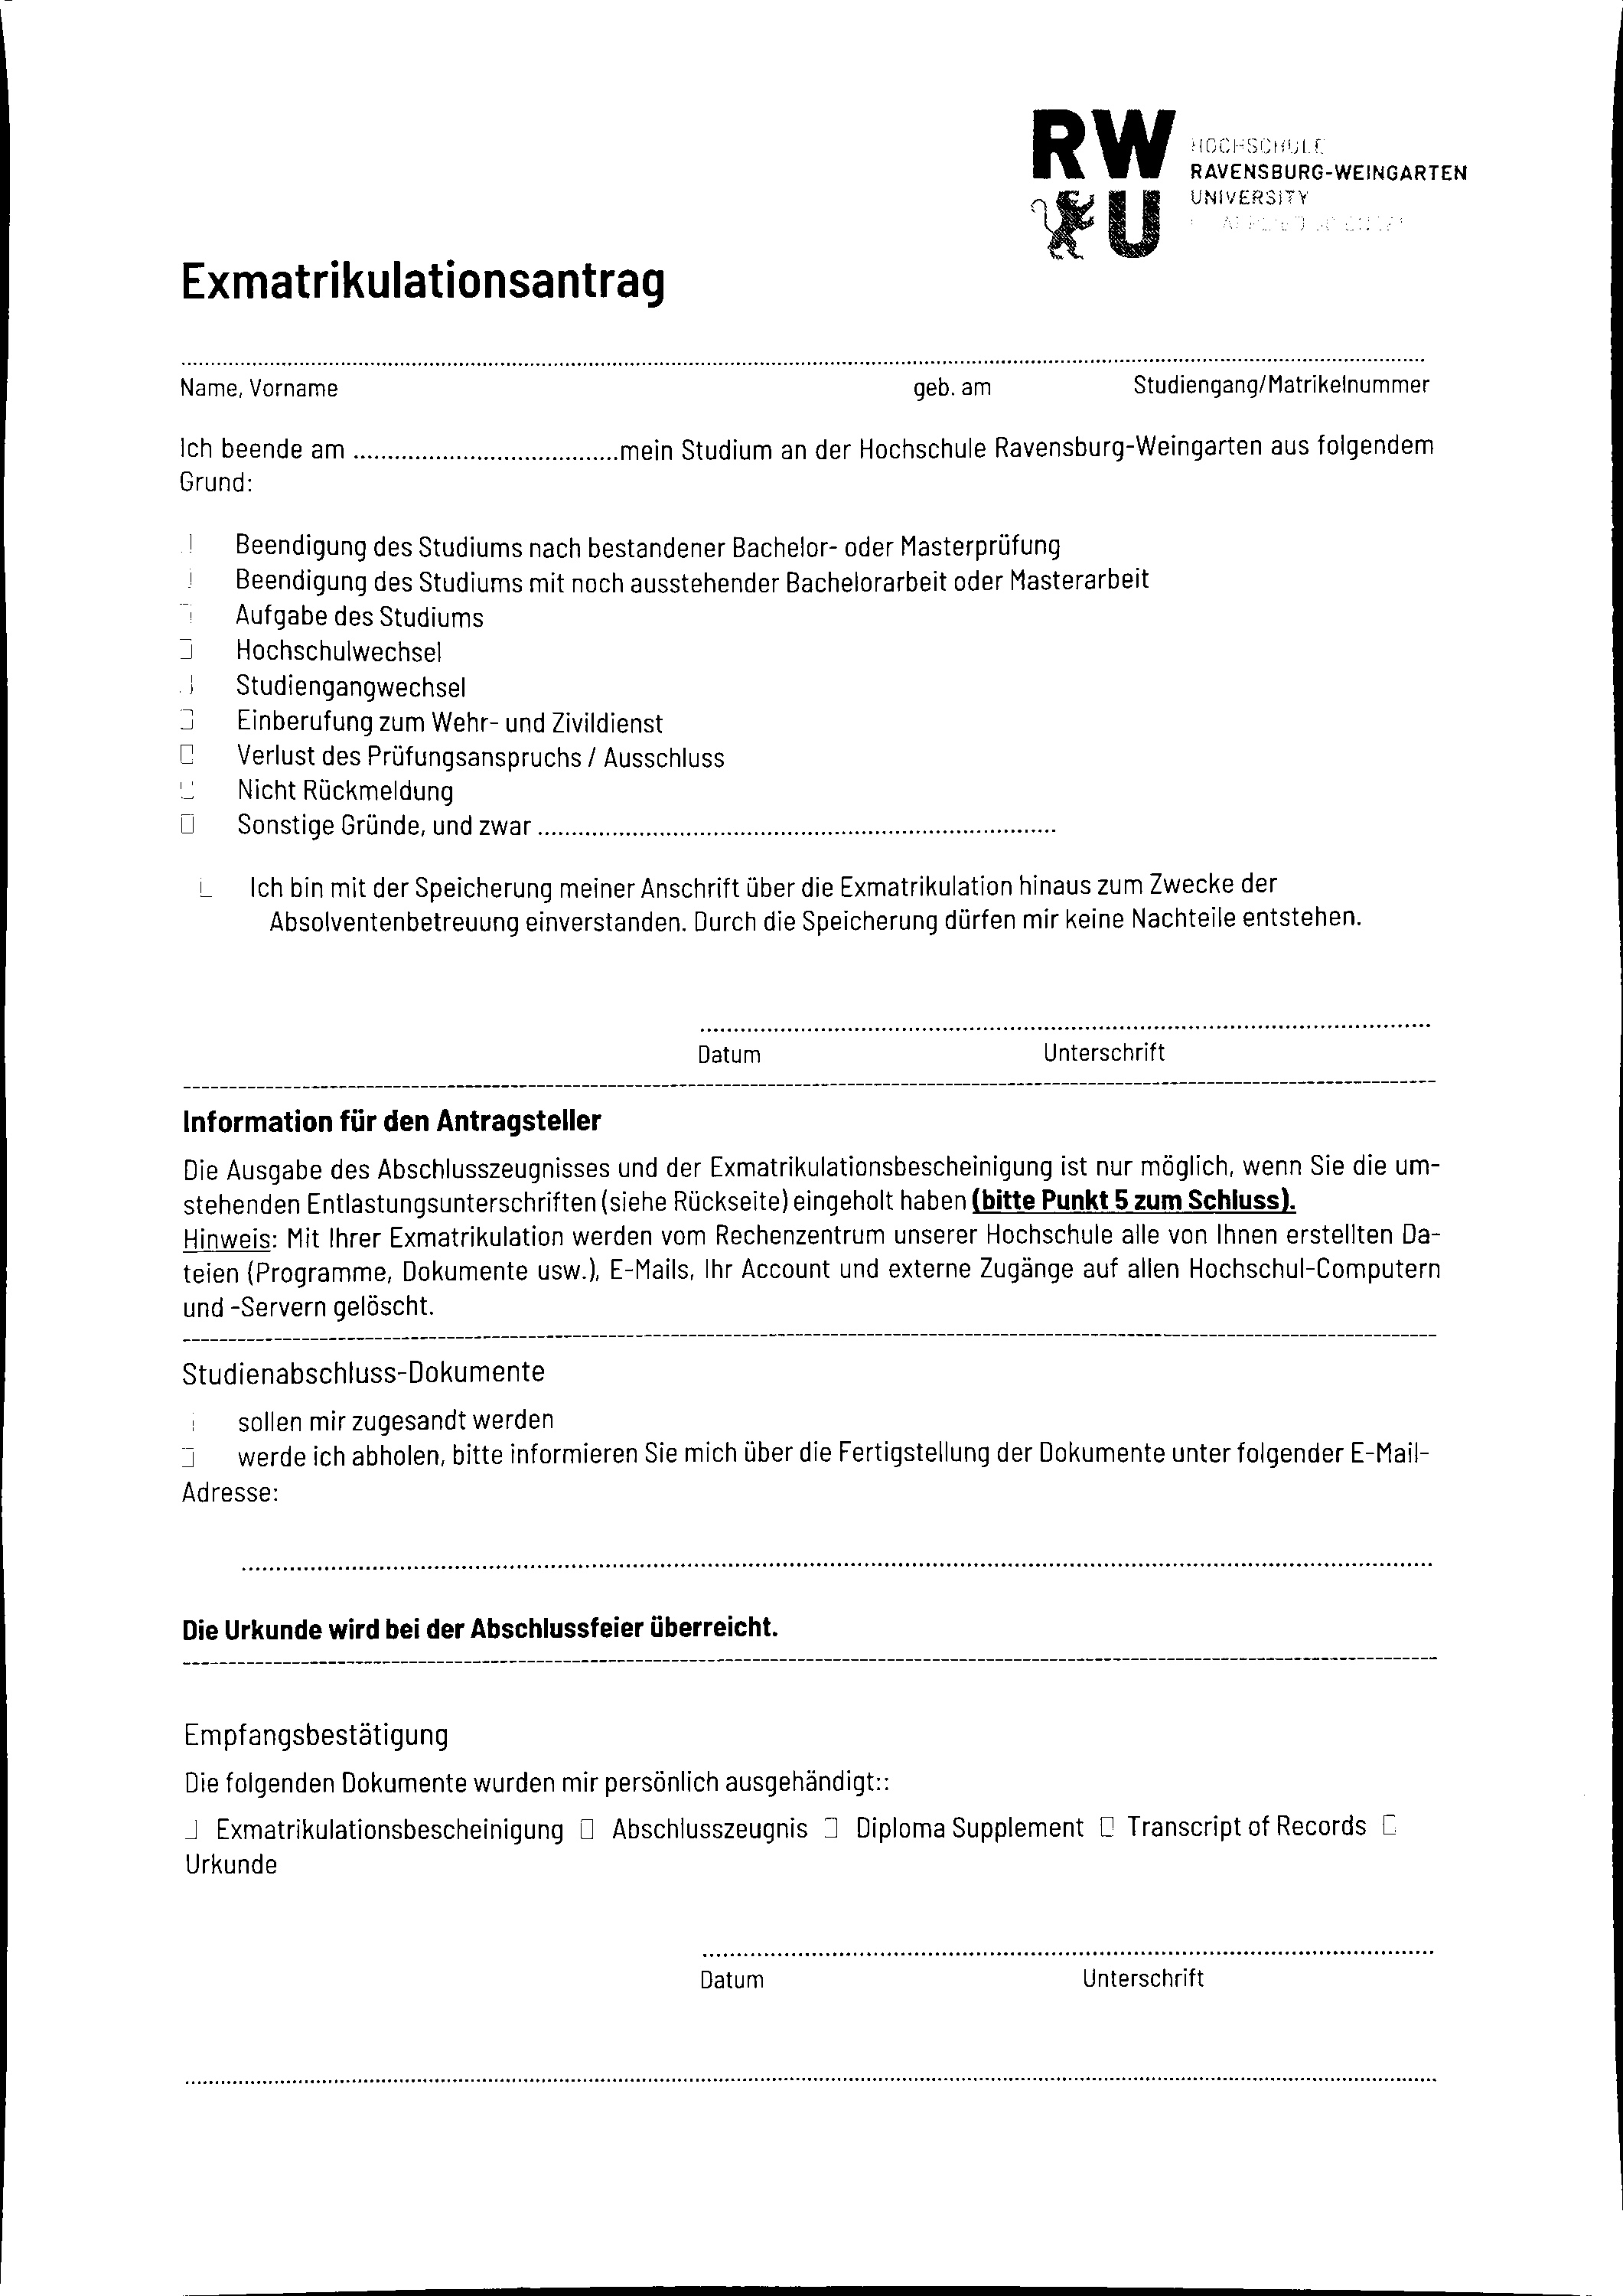
\includegraphics[width=2.5in]{output/hoch_3_9_binary_image.jpg}}
    \caption{The generated binary image.}
    \label{fig:binary}
\end{figure}
%The threshold value T(x,y) is a mean of the 𝚋𝚕𝚘𝚌𝚔𝚂𝚒𝚣𝚎×𝚋𝚕𝚘𝚌𝚔𝚂𝚒𝚣𝚎 neighborhood of (x,y) minus C

\section{Summary}
\noindent
% Ergebnisse mit beispielen
The example within the report and the two other examples attached below (Figures \ref{fig:schraeg2_original},\ref{fig:schraeg2_binary},\ref{fig:hoch1_original},\ref{fig:hoch1_binary}) show that the scanner does work even if the document is recorded in portrait or landscape format. The pictures of the documents show a small problem, that the recorded documents were wavy. Therefore the output documents show a wavy edge, but the content is still perfectly readable. The image of document of Figure \ref{fig:schraeg2_original} is even worse readable than the transformed document seen in Figure \ref{fig:schraeg2_binary}.\\\\
For further optimization it would be possible to add a character recognition to find out the real orientation of the document. This would fix the cases when the document has landscape format or is upside down and the assumptions 2 and 3 in the section \nameref{section:transformation} didn't have to be made.


\begin{figure}[H]
    \centerline{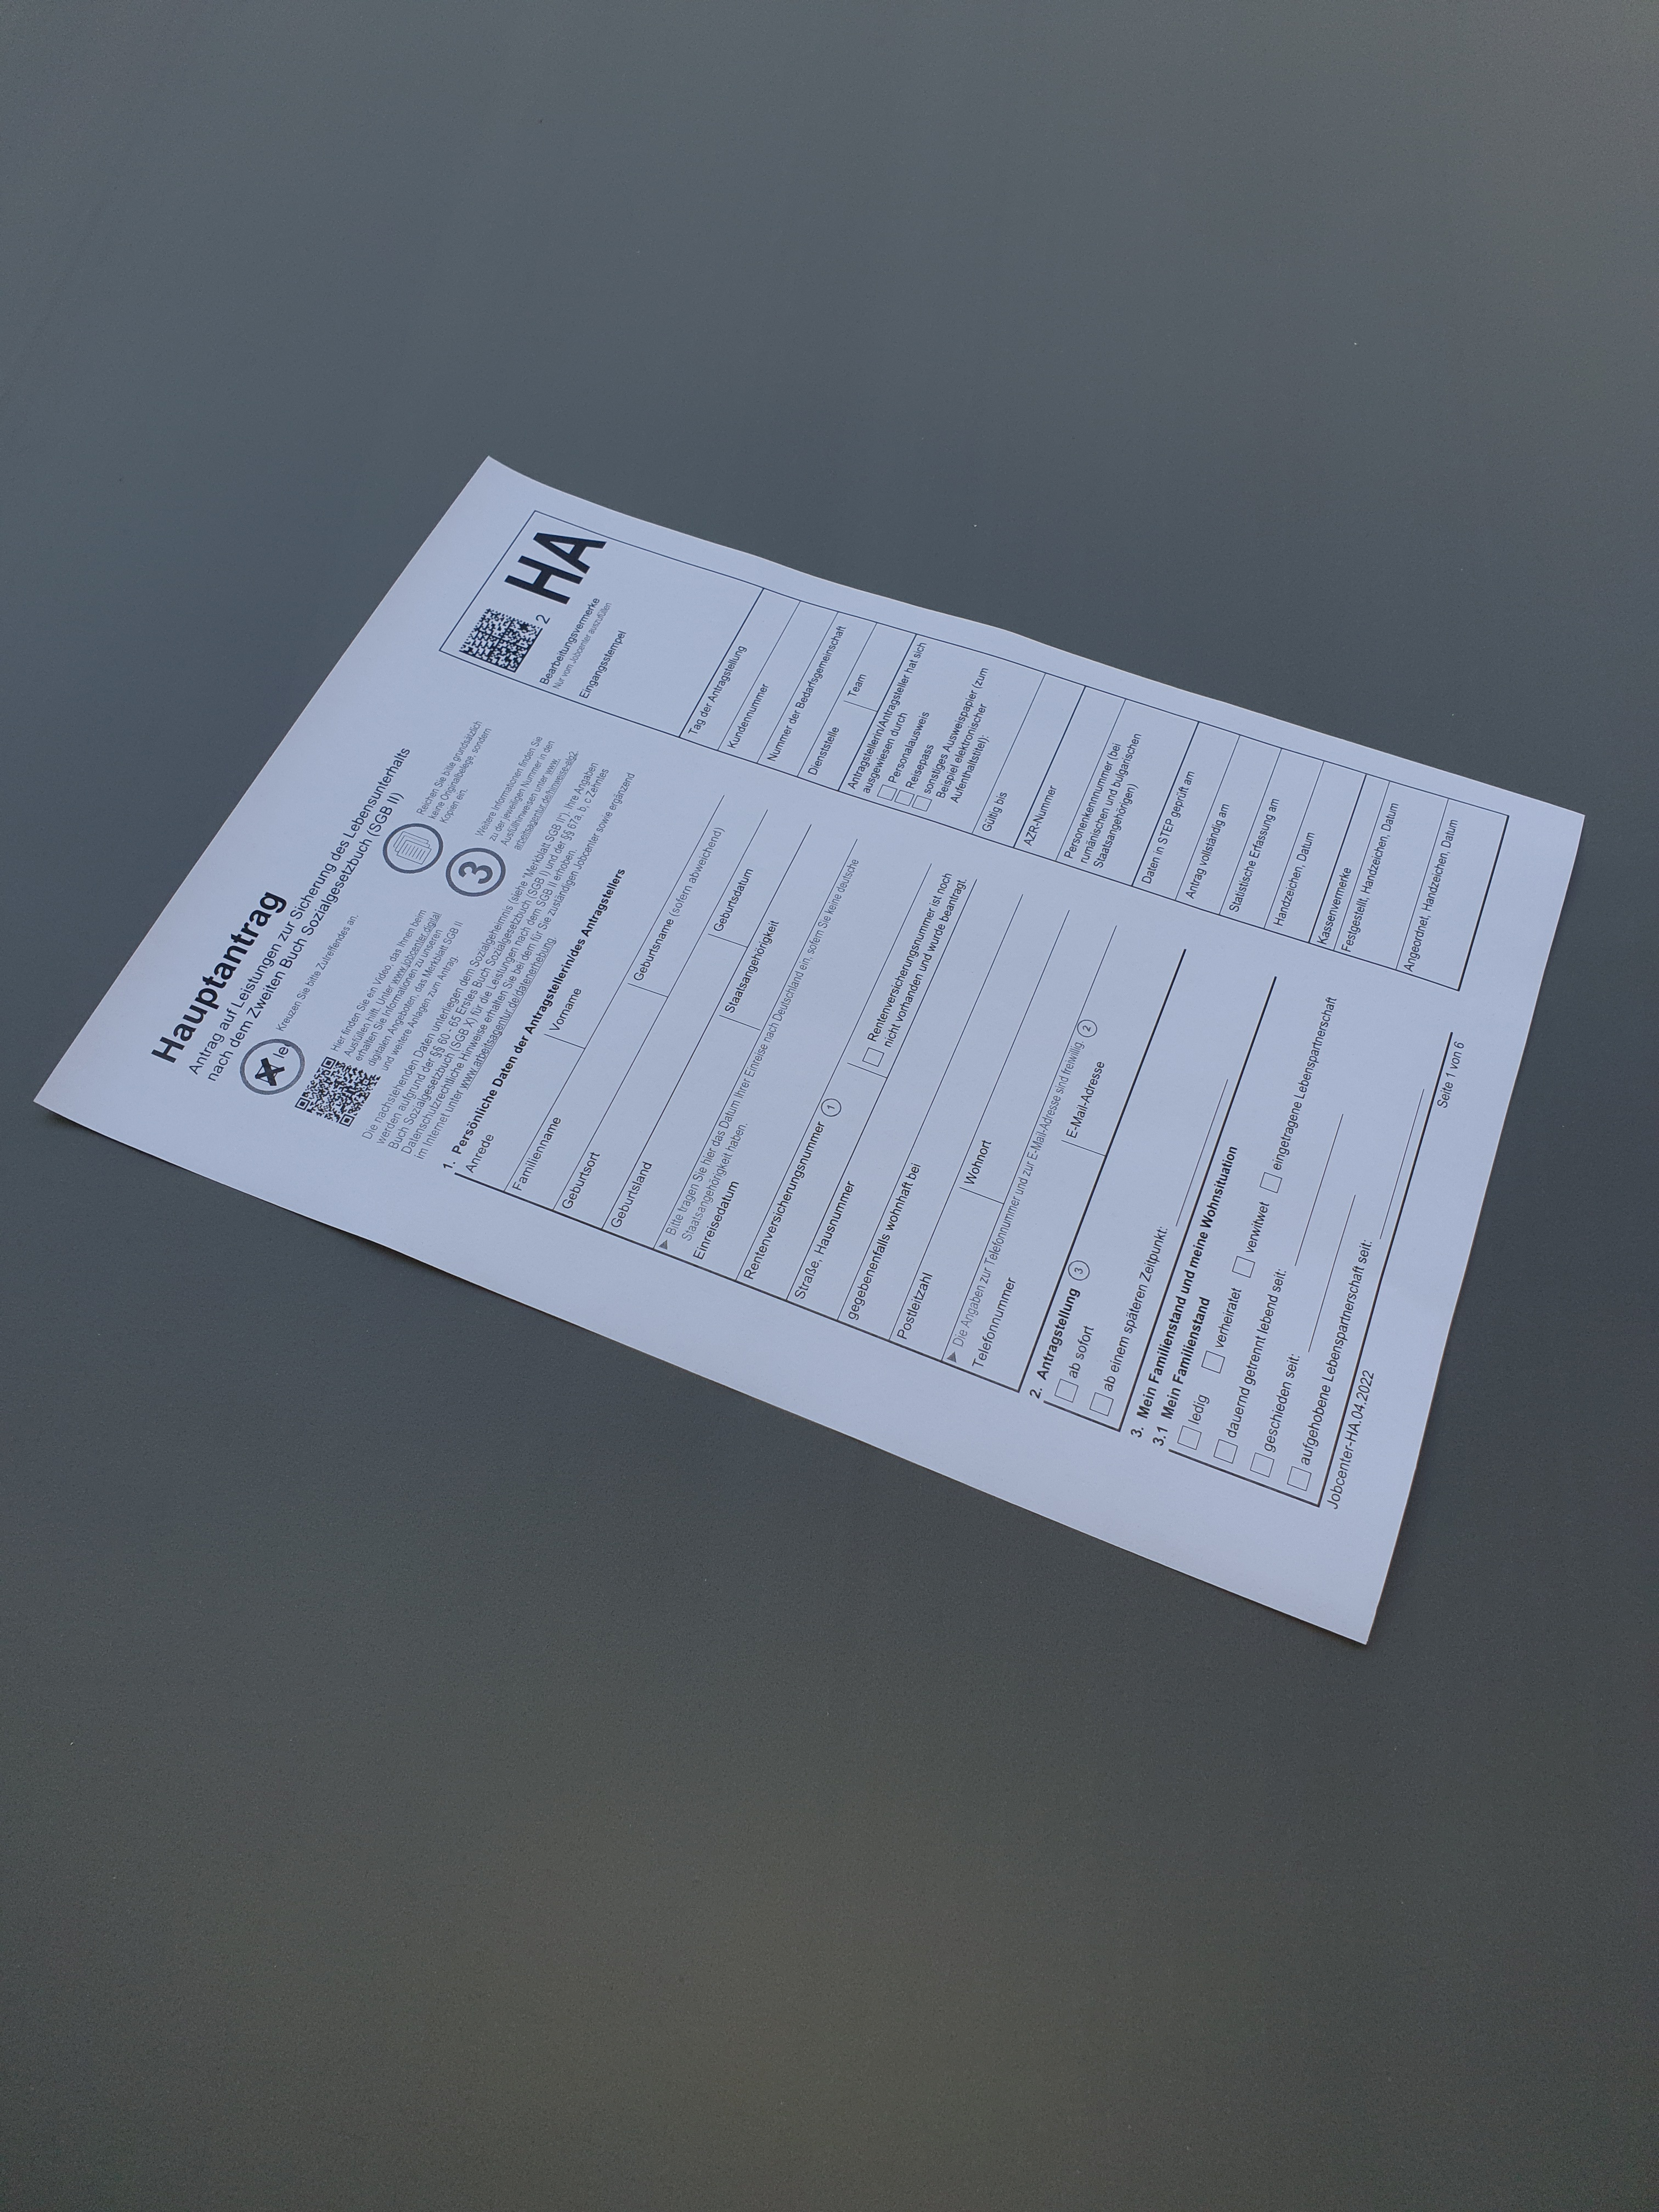
\includegraphics[width=2.5in]{output/schraeg_2_1_original.jpg}}
    \caption{Document recorded in landscape.}
    \label{fig:schraeg2_original}
\end{figure}

\begin{figure}[H]
    \centerline{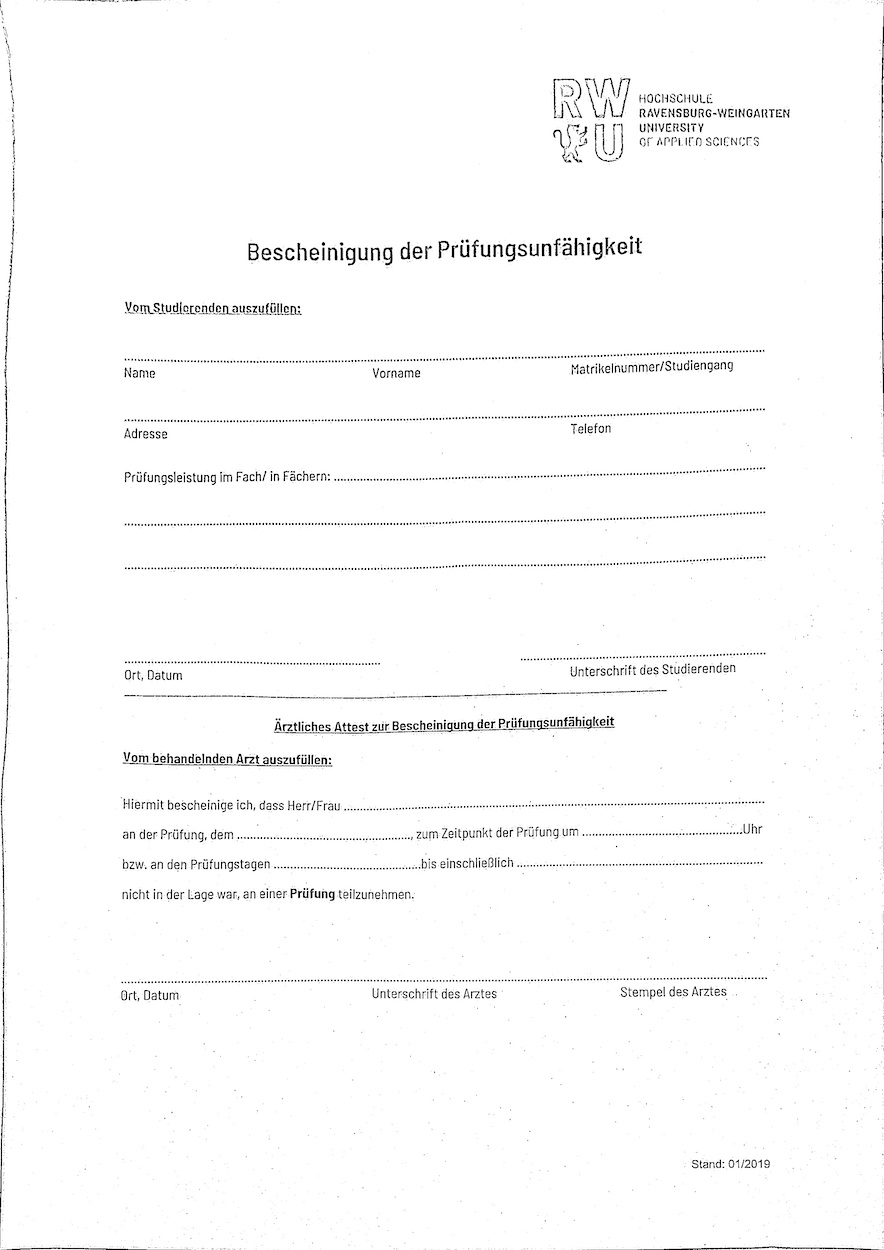
\includegraphics[width=2.5in]{output/schraeg_1_8_adaptive_binary_image_mean.jpg}}
    \caption{Document recorded in landscape transformed into binary document}
    \label{fig:schraeg2_binary}
\end{figure}

\begin{figure}[H]
    \centerline{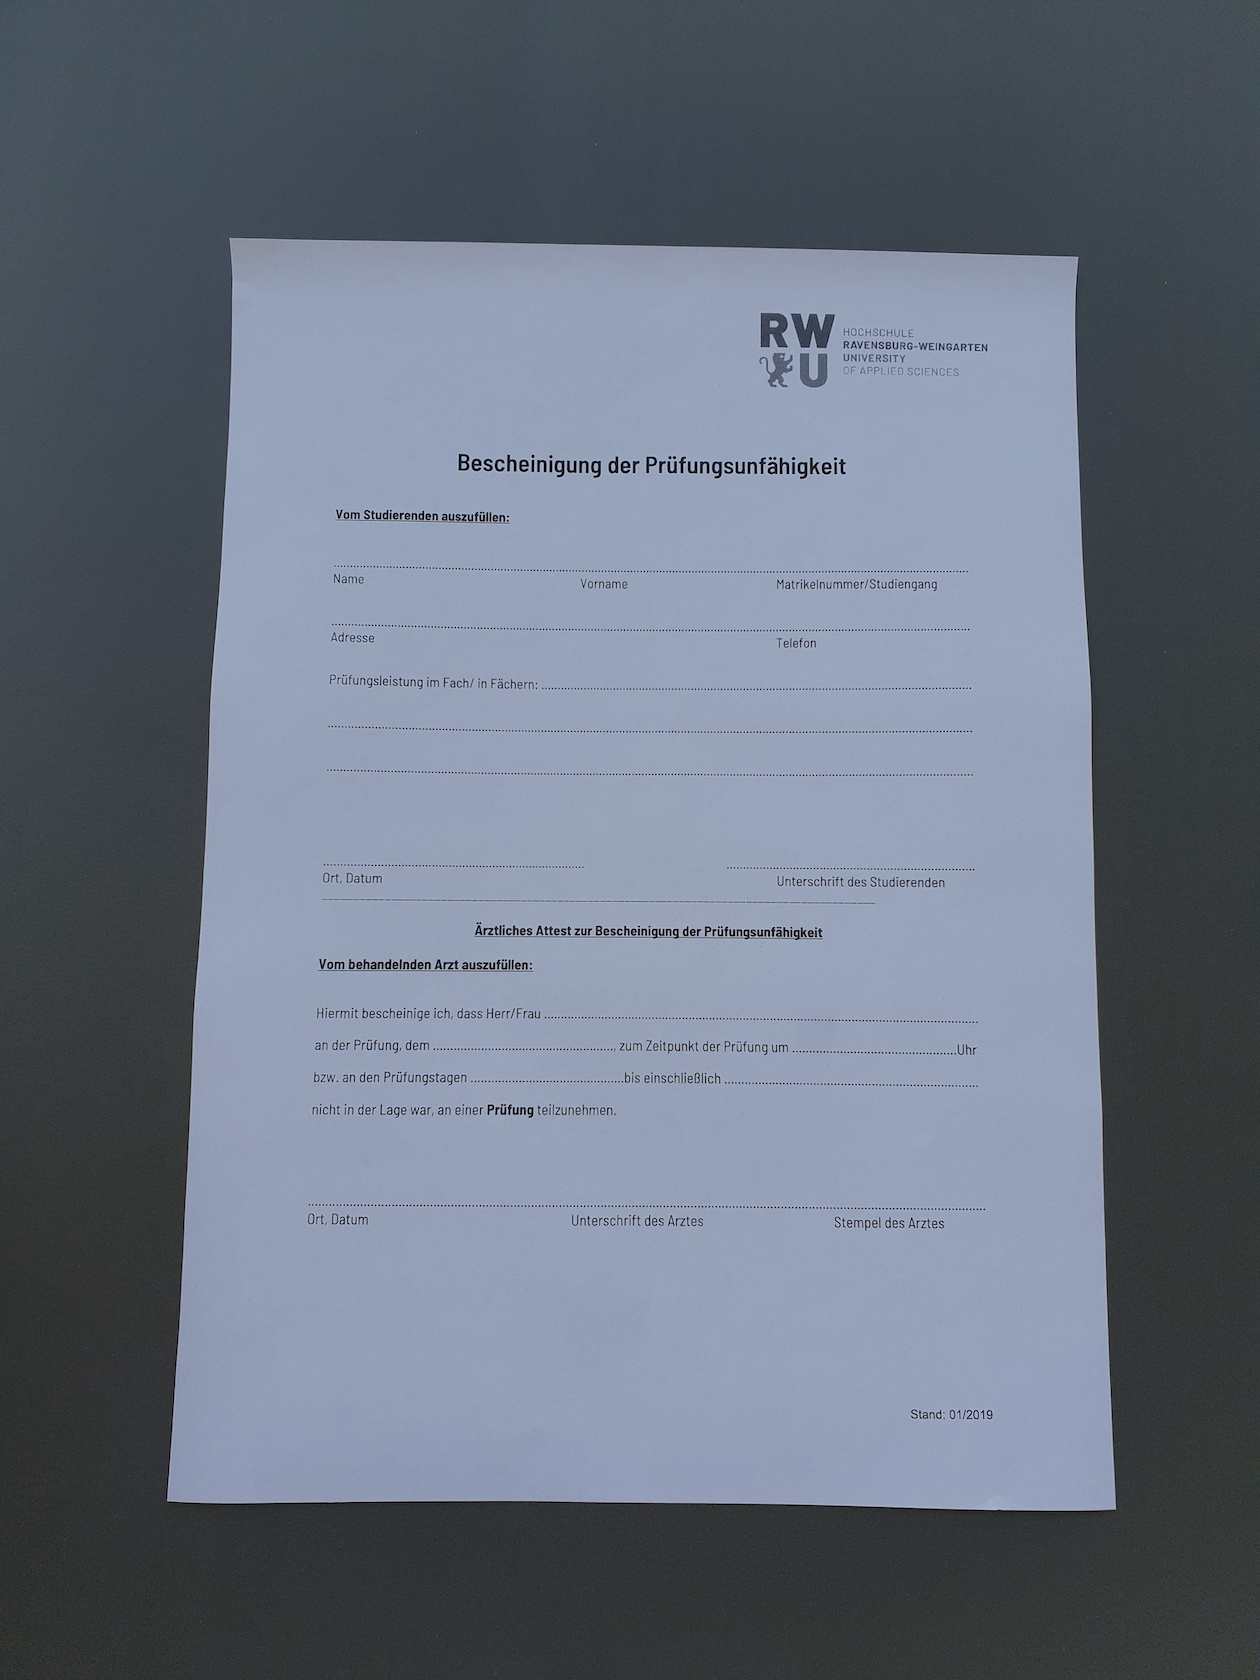
\includegraphics[width=2.5in]{output/hoch_1_1_original.jpg}}
    \caption{Document recorded in landscape.}
    \label{fig:hoch1_original}
\end{figure}

\begin{figure}[H]
    \centerline{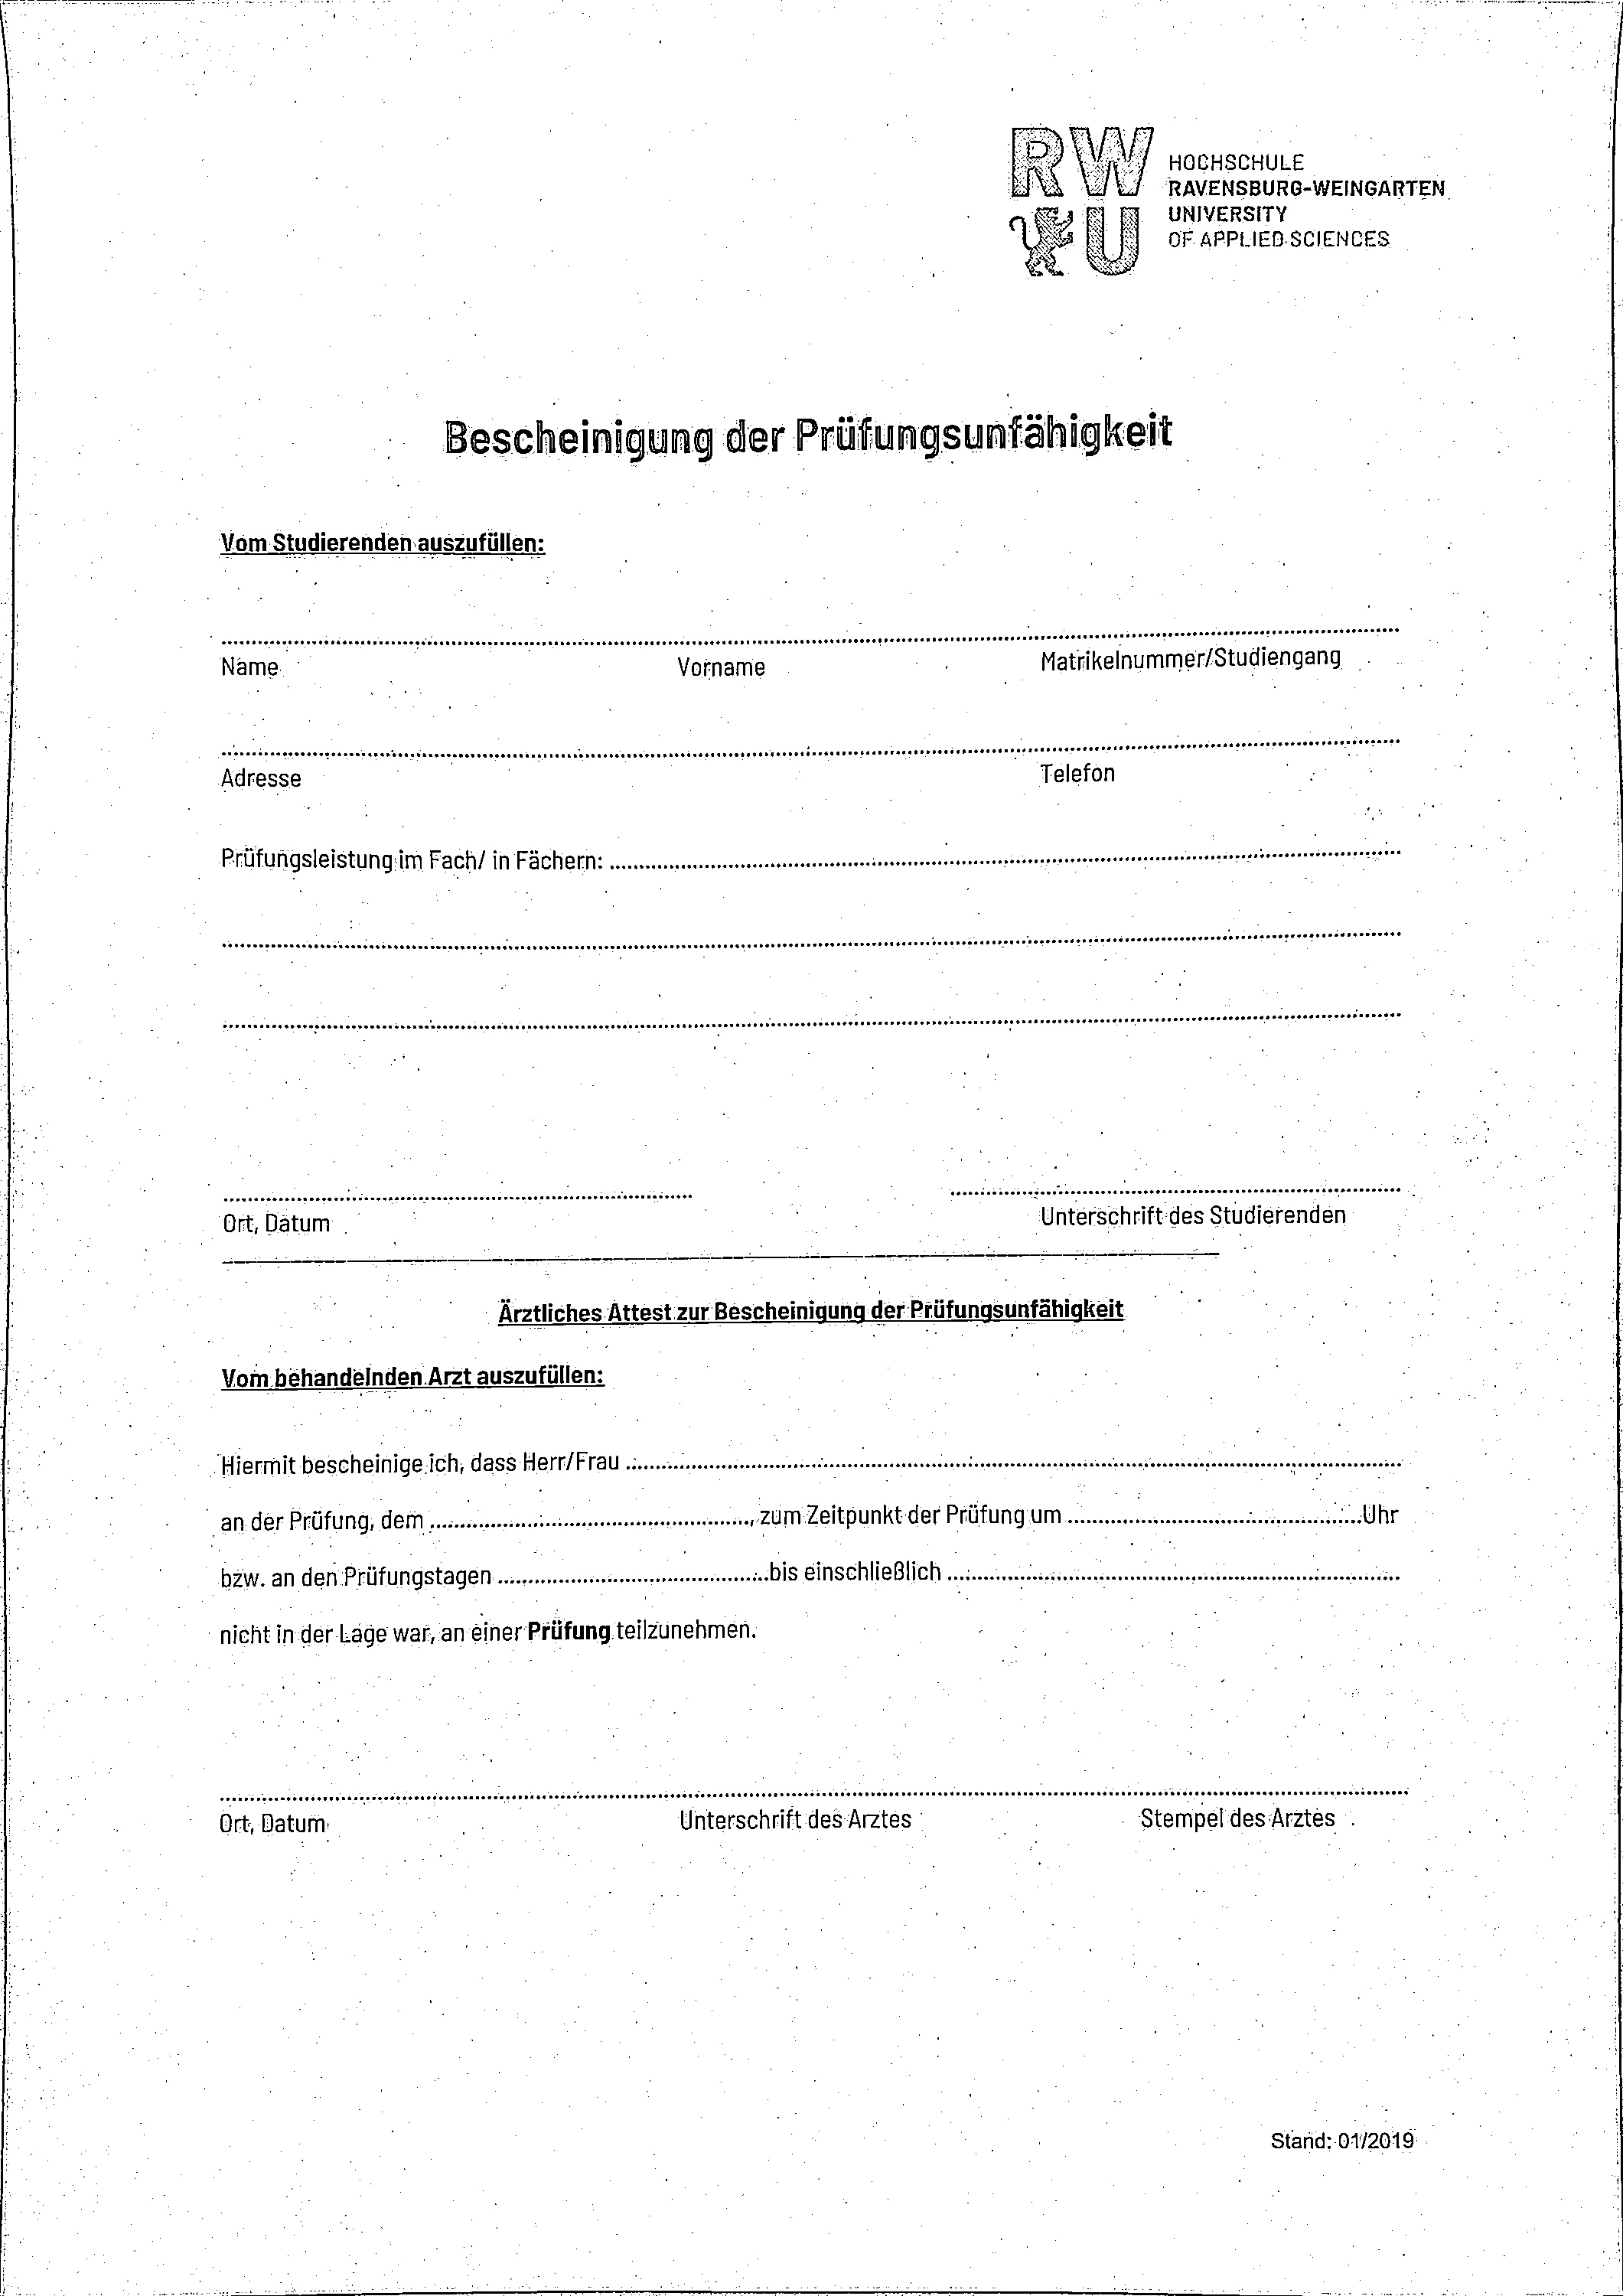
\includegraphics[width=2.5in]{output/hoch_1_8_adaptive_binary_image_mean.jpg}}
    \caption{Another document example transformed into binary document}
    \label{fig:hoch1_binary}
\end{figure}


% % Here's where you specify the bibliography style file.
% % The full file name for the bibliography style file 
% % used for an ASME paper is asmems4.bst.
% \bibliographystyle{asmems4}
\bibliographystyle{alpha}

% Here's where you specify the bibliography database file.
% The full file name of the bibliography database for this
% article is asme2e.bib. The name for your database is up
% to you.
\bibliography{asme2e}


\end{document}
